% % \part{优化模型}
% % \chapter{无约束非线性规划}

% \documentclass[UTF8]{ctexbook}

% \ctexset{
%     part/number = \chinese{part}
% }
% \usepackage{multirow}
% \usepackage{amsmath}% ams 数学公式
% \usepackage{amsfonts}% ams 数学字体
% \usepackage{bbm}%重影字体
% \usepackage{amssymb,latexsym}% ams 数学符号与LaTeX数学符号
% \usepackage{mathrsfs}% 花式符号
% \usepackage{ntheorem}%定理、定义、证明
%     \theoremstyle{nonumberplain}
%     \theoremheaderfont{\bfseries}
%     \theorembodyfont{\normalfont}
%     \theoremsymbol{$\square$}
%     \newtheorem{Proof}{\hskip 2em 证明}
%     \newtheorem{theorem}{\hspace{2em}定理}[chapter]
%     \newtheorem{definition}{\hspace{2em}定义}[chapter] % 如果没有章, 只有节, 把上面的[chapter]改成[section]
%     \newtheorem{axiom}[definition]{\hspace{2em}公理}
%     \newtheorem{lemma}[definition]{\hspace{2em}引理}
%     \newtheorem{proposition}[definition]{\hspace{2em}命题}
%     \newtheorem{corollary}[definition]{\hspace{2em}推论}
%     \newtheorem{remark}{\hspace{2em}注}[chapter] %类似地定义其他“题头”. 这里“注”的编号与定义、定理等是分开的
%     \newtheorem{Assumption}{\hspace{2em}假设}[chapter]

% %算法伪代码
% %http://blog.csdn.net/lwb102063/article/details/53046265
% \usepackage{algorithm}
% \usepackage{algorithmicx}
% \usepackage{algpseudocode}
%     \floatname{algorithm}{算法}
%     \renewcommand{\algorithmicrequire}{\textbf{输入:}}
%     \renewcommand{\algorithmicensure}{\textbf{输出:}}
% % 罗马数字:示例:\rom{2}
% \makeatletter
% \newcommand*{\rom}[1]{\expandafter\@slowromancap\romannumeral #1@}
% \makeatother

% \usepackage{enumerate}%itemiz环境。\begin{enumerate}[step 1][a)]可以使用 A,a,I,i,1 作为可选项产生 \Alph,\alph,\Roman,\roman,\arabic 的效果
% \usepackage{cite}%参考文献
%     \bibliographystyle{plain}
% \usepackage{extarrows}% 带参数的箭头
% \usepackage{hyperref}% 超链接
% \usepackage{pifont}%然后在正文输入\ding{172}~\ding{211}得到相应数字,要是要①就输入:\ding{172}②就输:\ding{173}
% %\usepackage[CJKbookmarks, colorlinks, bookmarksnumbered=true,pdfstartview=FitH,linkcolor=black,citecolor=black]{hyperref}%超链接的格式设置
% \hypersetup{
%     colorlinks=false,% 去掉超链接颜色
%     pdfborder=0 0 0% 取消超链接的边框
% }
% \usepackage{graphicx}% 图片管理
% \usepackage{caption}
% \usepackage{subcaption}%并排的图各有标题
% \graphicspath{{images/}}% 设置图片搜索路径
% \usepackage{float,varwidth}% 浮动体
% \usepackage{booktabs}% 三线表
% \usepackage{fancyhdr}% 页眉设置
% \usepackage{xcolor}% 颜色宏包
% \usepackage{colortbl}% 彩色表格
% \usepackage{listings}% 代码高亮
% \usepackage{caption}% 对标题进行控制,如让\caption标题的字体缩小一号,同时数字标签使用粗体可以用:\usepackage[font=small,labelfont=bf]{caption}
% \usepackage{xfrac,upgreek}%分别是行间公式如a/b的形式(将原来的命令\frac改成\sfrac)和希腊字体的宏包的
% \usepackage{mathtools}%lgathered和rgathered环境把公式向左向右对齐
% \usepackage{tabularx}%提供自动延伸的表列,(X列格式说明符),文字过长时可以自动转行
% \usepackage{longtable}%长表格
% \usepackage{enumitem}%enumerate宏包的升级
% \usepackage{harpoon}%数学公式的矢量
% \usepackage{bookmark}%目录的书签
% \renewcommand{\headwidth}{\textwidth}%图片并排,这个要列在所有宏包的后面
% \definecolor{codegreen}{rgb}{0,0.6,0}
% \definecolor{codegray}{rgb}{0.5,0.5,0.5}
% \definecolor{codepurple}{rgb}{0.58,0,0.82}
% \definecolor{backcolour}{rgb}{0.95,0.95,0.92}
% \lstset{
%     commentstyle=\color{codegreen},
%     keywordstyle=\color{magenta},
%     numberstyle=\tiny\color{codegray},
%     stringstyle=\color{codepurple},
%     basicstyle=\footnotesize,
%     breakatwhitespace=false,% 断行只在空格处
%     breaklines=true,% 自动断行
%     captionpos=b,% 标题位置
%     keepspaces=true,
%     numbers=left,
%     numbersep=5pt,
%     showspaces=false,
%     showstringspaces=false,
%     showtabs=false,% 显示
%     tabsize=2% TAB 被当作两个空格
% }
% \topmargin=0pt\oddsidemargin=0pt\evensidemargin=0pt
% \textwidth=16.5cm\textheight=23cm\raggedbottom%我这么设置是为了缩小页边距,满足有的文字无法转行
% \pagestyle{headings}%页眉为章节标题,无页脚
% \setlength{\abovecaptionskip}{10pt}
% \setlength{\belowcaptionskip}{-15pt}%图片表格的前后距离设置
% \CTEXsetup[format={\zihao{-3}\raggedright\bfseries}]{section}%设置节的格式

% \begin{document}
% \part{优化模型}
\chapter{无约束非线性规划}
\section{引言}
    \par
    许多模型(如支持向量机,线性回归等)最终都会转化为一个优化问题。这是因为我们在处理问题时,总是希望在众多可选择的情况中选择最优的。回想一下,在数学分析中的优化问题:我们会求一个函数$f(x)$的极大值、极大值点、最大值、最大值点等等。又或者,我们在“Lagrange乘子法”中讨论了在等式约束“$h(x)=0$”下$f(x)$最优化。现在,我们将这些所谓的函数“放宽”:我们希望在“一类事物”中,找到某个指标下的最优个体(或者最优群体)。明显,这一类事物应该是一个集合。不妨记集合为$\phi$,集合中的个体$x$的特点(特征)记为$I(x)$。
    \par
    当然,我们不能一眼看出来集合中哪个个体最好,所以,我们需要东奔西跑的去找。但是,我们一般不会盲目的去寻找。我们将寻找最优解(个体)的方法分为有指导(有方向)的寻找和随机性寻找以及二者相结合的3大类方法。这种寻找过程(优化算法)必然是一步一步反复迭代的:这一步找到了张三,下一步找到了李四,最终找到最优结果。有指导寻找:$A \rightarrow B \rightarrow \cdots$;随机寻找:$A,C,F,\cdots$。一个显著的特点是:有指导的寻找应该是现在的结果比上一次要好,随机则不一定,而二者的结合方法亦不确定。
    \par
    我们不可能设计一个算法(寻找方法),说这个算法对所有优化问题都适用,毕竟各种优化问题会有它自身的特点,因此要具体问题具体分析。后面,我们将在分析具体的某一类优化问题时,给出其适应的算法。
\section{问题的引入与分析}
    \par
    考虑如下不含参数的无约束非线性优化问题
    \begin{align}\label{tab:不含参的无约束非线性优化}
    {\min \limits_{x \in {R^2}} f(x)} = x_1 \exp(-(x_1^2 +x_2^2))
    +{(x_1^2 +x_2^2)/{20}}
    \end{align}
    在上述优化问题中外加参数,形成如下含参数的无约束非线性规划问题
    \begin{align}\label{tab:含参的无约束非线性优化}
    {\min \limits_{x \in {R^2}} f(x;a,b,c)} = ({x_1} - a)\exp(-(x_1-a)^2+ (x_2-b)^2)
    + {((x_1-a)^2 + (x_2-b)^2)/{c^2}}
    \end{align}
    其中:$x=(x_1,x_2) \in R^2$,$a,b,c$为参数。我们的目标是寻找$x=(x_1,x_2)\in R^2$,使得$f(x)$最小。
    \par
    在MATLAB中,Optimization Toolbox使用下面3种方法求解上述无约束非线性最小化问题:
    \begin{enumerate}
        \item 拟牛顿法:使用二次或三次线搜索技术并使用BFGS公式来计算海赛矩阵;
        \item Nelder-Mead算法:只使用目标函数值来直接寻找最优点,可用于处理非平滑目标函数;
        \item 信赖域法:特别适用于有稀疏矩阵或其他结构的大规模问题。
    \end{enumerate}
    \par
    用MATLAB解上述问题(\ref{tab:含参的无约束非线性优化}):
    \begin{lstlisting}[language=Matlab]
    y = @(x,a,b,c)
    (x(1)-a).*exp(-((x(1)-a).^2+(x(2)-b).^2))+((x(1)-a)^2+(x(2)-b)^2)/c;
    a = 0;
    b = 0;
    c = 20;
    obj = @(x)y(x,a,b,c);
    e2surfc(obj, [-2,2]);
    x0 = [-0.5;0];
    options = optimset('fminunc', 'Algorithm', 'quaci–newton')
    options.Display = 'iter'; %点索引
    [x, fval, exitflag, output] = fminunc(obj, x0, options)
    %% 绘制等高线图以及迭代动图
    \end{lstlisting}
\section{模型规范化及基本理论}
    \par
    将前面的例子(\ref{tab:不含参的无约束非线性优化})和(\ref{tab:含参的无约束非线性优化})忽略参数,写成一般形式
    \begin{align*}
    {\min \limits_{x \in {R^n}} f(x)}
    \end{align*}
    \par
    上式即为无约束非线性优化的一般形式,我们的目标是在$x \in R^n$中求最优$x^*$,使得$f$最小。我们在数学分析中已经学过当$n=1,2,3$时,某些特定的$f$的极值点的求解。要注意的是,我们是求某一类型的$f$(如$f$连续可微)的极值点而并非任何一个$f$。下面,我们将在$R^n$中讨论$f(x)$极值问题。
    \subsection{点的性质}
        \par
        首先,我们给出$n$维空间$R^n$中点$x$的一些定义:
        \begin{definition}[半范数]
        定义映射$\|\cdot \|:R^n \rightarrow R$为$R^n$上的半范数,当且仅当它具有如下性质
        \par
        (i) $\| x \| \ge 0,\forall x \in {R^n}$;
        \par
        (ii) $\| \alpha x \| =|\alpha| ||x||, \forall\alpha \in R,\forall x \in {R^n}$;
        \par
        (iii) $\| x+y \|  \le \| x \| + \| y\|, \forall x,y \in {R^n}$。
        \end{definition}
        \begin{definition}[范数]
        映射$\|\cdot \|:R^n \rightarrow R$为$R^n$上的范数,当且仅当它是半范数,且
        \begin{align*}
          \|x \| = 0 \Leftrightarrow x=\theta
        \end{align*}
        其中:$\theta$为$R^n$中的$0$点。
        \end{definition}
        \par
        设$x=(x_1,x_2,\dots,x_n)^\mathrm{T} \in R^n$,常用的向量范数有
        \begin{align*}
        & \| x \|_\infty  = \mathop {\max }\limits_i |x_i| \quad (l_\infty \text{范数})\\
        & \| x \|_1 = \sum \limits_{i=1}^n |x_i| \quad (l_1 \text{范数})\\
        & \| x \|_2 = \sqrt{\sum \limits_{i=1}^n x_i^2} \quad (l_2 \text{范数})\\
        & \| x \|_p = \left( {\sum \limits_{i=1}^n} |x_i|^p \right) ^{\frac 1 {p}}  \quad (l_p \text{范数})
        \end{align*}
        \par
        类似于向量范数的定义,我们可以定义矩阵范数。设$A \in R^{m\times n}$,其诱导矩阵范数为
        \begin{align*}
        \|A\| = \mathop {\max }\limits_{x \ne 0} \bigg \{\frac {\|Ax\|}{\|x\|} \bigg \}
        \end{align*}
        其中:$\|x\|$是某一向量范数。特别地,有
        \begin{align*}
        & {\|A\|}_1= \mathop {\max} \limits_j\{{\|a_{\cdot j}\|}_1\} = \mathop {\max} \limits_j \sum \limits_{i = 1}^n |a_{ij}|\\
        & {\|A\|}_{\infty} = \mathop {\max} \limits_i \{{\|a_{i \cdot}\|}_1\} = \mathop {\max} \limits_i \sum\limits_{j = 1}^n |a_{ij}|\\
        & {\|A\|_2} = (\lambda_{ A^\mathrm{T}A})^{\frac 12}
        \end{align*}
        其中:$\lambda_{ A^\mathrm{T}A}$表示$A^\mathrm{T}A$的最大特征值,$a_{\cdot j}$表示$A$的第$j$列,$a_{i \cdot}$表示$A$的第$i$行。显然
        \begin{align*}
        & \|A^{-1}\| = {\frac 1{\|A\|}}\\
        & \|I\| = 1
        \end{align*}
    \subsection{目标函数的性质}
        \par
        下面来讨论某些特定的$f:R^n \rightarrow R$。首先,我们给出函数导数的定义。
        \begin{definition}[一阶导数]
        如果$\left( \frac {\partial f}{\partial x_i} \right) (x),i=1,2,\ldots,n$存在且连续,则函数$f:R^n \rightarrow R$在$x\in R^n$连续可微。如果$f$在开集$D\subset R^n$中的每一点连续可微,则称$f$在$D$中连续可微,记为$f \in C^1 (D)$。定义$f$在$x$处的梯度为
        \begin{align*}
            g = \nabla f(x) = \bigg[{\frac{\partial f}{\partial x_1}}(x), \cdots ,{\frac{\partial f}{\partial x_n}}(x)\bigg]^\mathrm{T}
        \end{align*}
        \end{definition}
        \begin{definition}[二阶导数]
        如果$\left( \frac {\partial^2 f}{\partial x_i\partial x_j} \right) (x),i=1,2,\ldots,n$存在且连续,则函数$f:R^n \rightarrow R$在$x\in R^n$二次连续可微。如果$f$在开集$D\subset R^n$中的每一点二次连续可微,则称$f$在$D$中二次连续可微,记为$f \in C^{2}(D)$。定义$f$在$x$处的Hessian矩阵为
        \begin{align*}
        G = [\nabla ^2f(x)]_{ij} = \frac{\partial f(x)}{\partial {x_i}\partial {x_j}}  \quad 1\le i,j \le n
        \end{align*}
        \end{definition}
        \par
        设$f:R^n \rightarrow R$在开集$D\subset R^2$上连续可微。对于$x\in R^n,d\in R^n$,$f$在$x$点关于方向$d$的方向导数定义为
        \begin{align*}
        \frac{\partial f}{\partial d}(x) = \mathop {\lim }\limits_{\theta \to 0} \frac{f(x+\theta d)-f(x)}{\theta }
        \end{align*}
        上述定义的方向导数等于$\nabla {f(x)}^\mathrm{T} d$。其中,$\nabla {f(x)}$为梯度,它是$f$的导数$f'(x)$的转置,是$n \times 1$向量。
        \par
        设$f:R^n \rightarrow R$在开集$D\subset R^2$上连续可微,对于$x\in R^n,d\in R^n$,$f$在$x$点关于方向$d$的方向导数定义为
        \begin{align*}
        \frac{{\partial}^2 f}{\partial d^{2}}(x) = \mathop {\lim }\limits_{\theta \to 0} \frac{{\frac {\partial f}{\partial d}}(x+\theta d)-{\frac {\partial f}{\partial d}}(x)}{\theta }
        \end{align*}
        上述定义的二阶方向导数等于$d^\mathrm{T}{\nabla^2} f(x) d$。其中,${\nabla^2} f(x)$是$f$在$x$点的Hessian矩阵。
    \subsection{最优性条件}
        \par
        上面给出了向量(矩阵)范数、$f$连续可微、二次连续可微的定义。下面,我们将在这些定义的基础上给出无约束非线性优化问题的最优性条件。
        \par
        回到我们前面的目标:求$x \in R^n$,使$f(x)$最小。我们自然会问:什么是最小,什么情况下最小(极小值存在性)。首先,我们给出极小值的两种类型的定义:局部极小点和总体极小点。$f:x \in R\to R$的极小点类型示意图如图(\ref{极小点类型示意图})所示
        \begin{figure}[H]
        \centering
        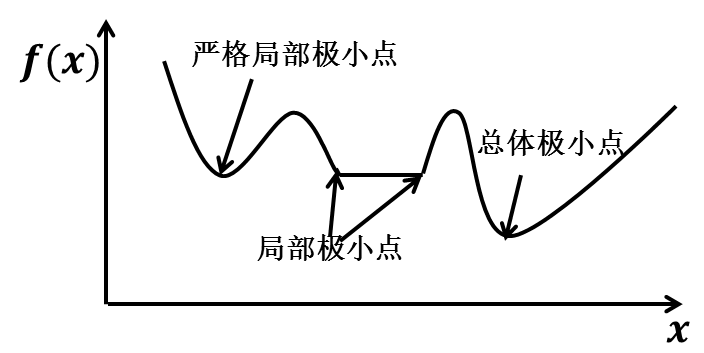
\includegraphics[height=3cm]{images/Minimal_point.jpg}
        \caption{极小点类型示意图}
        \label{极小点类型示意图}
        \end{figure}
        % \textcolor[rgb]{1,0,0}{todo:图片:极小点类型示意图}
        \begin{definition}[局部极小点]
          如果$\exists f >0,\forall x \in N(x^{*},\delta) = \{x \in R^n |\|x-x^{*}\|<\delta)\}$,有
          \begin{align*}
            f(x^{*}) \leqslant f(x)
          \end{align*}
          则称$x^{*}$为$f$的一个局部极小点。
          若$f(x^{*})<f(x)$且$x \ne x^{*}$,则称$x^{*}$为$f$的一个严格局部极小点。
        \end{definition}
        \begin{definition}[总体极小点]
          如果$\forall x \in R^n$都有
          \begin{align*}
            f(x^{*}) \leqslant f(x)
          \end{align*}
          则称$x^{*}$为$f$的一个总体极小点。
          若$f(x^{*})<f(x)$且$x \ne x^{*}$,则称$x^{*}$为$f$的一个严格总体极小点。
        \end{definition}
        \par
        应该指出,实践中,我们只是求一个局部极小点而非全局(总体)极小点,因为总体极小点往往是难以求解的。后面大部分章节讨论局部极小点,在全局优化及智能优化中讨论的是全局极小点。并且,应当注意的是:当问题具有某种凸性时,局部极小点就是总体极小点。
        % 如下图(\ref{fig:凸函数的极小点示意图})所示
        % \begin{figure}[H]
        % \centering
        % 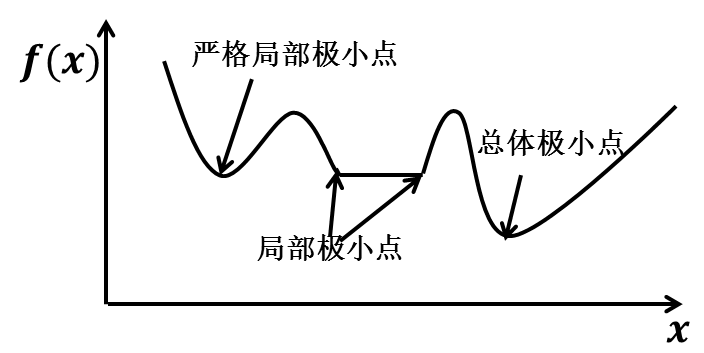
\includegraphics[height=3cm]{images/Minimal_point.jpg}
        % \caption{凸函数的极小点示意图}
        % \label{fig:凸函数的极小点示意图}
        % \end{figure}
        % \textcolor[rgb]{1,0,0}{todo:图片:凸函数的极小点示意图}
        \par
        下面给出(局部)极小点存在的充分必要条件(即最优性条件/极小点解的存在性)。为方便书写,记
        \begin{align*}
        & g(x) = \nabla f(x),g_k=\nabla f(x_k)\\
        & G(x)={\nabla^2} f(x),G_k={\nabla^2} f(x_k)
        \end{align*}
        \par
        \textbf{一阶必要条件}:设$f:D\subset R^n \to R$在开集$D$上连续可微。若$x^{*} \in D$是局部极小点,则
        \begin{align*}
          g(x^{*}) = 0
        \end{align*}
        \par
        \textbf{二阶必要条件}:设$f:D\subset R^n \to R$在开集$D$上二次连续可微。若$x^{*} \in D$是局部极小点,则
        \begin{align*}
          g(x^{*}) = 0,\quad G(x^*) \ge 0
        \end{align*}
        \par
        \textbf{二阶充分条件}:设$f:D\subset R^n \to R$在开集$D$上二次连续可微($f \in C^2(D)$),若$g(x^{*})=0$并且$G(x^{*})$是正定矩阵,则$x^{*} \in D$是$f$的一个严格极小点。
        \par
        一般的,目标函数的稳定点($g(x)=0$)不一定是极小点。但当$f$为凸函数时,其稳定点、局部极小点和总体极小点是等价的。
        \par
        设$f:R^n \to R$是凸函数,且$f \in C^{1}$,则$x^{*}$是总体极小点的充分必要条件是$g(x^{*})=0$。
\section{算法框架}
    \par
    最优化方法通常采用迭代方法进行求解。我们给定一个初始点$x_0$,然后按照某一方向以某个大小的步子去靠近$x^{*}$。当然,我们会迭代许多次以靠近$x^{*}$。在这个过程中会产生一系列的点,我们将其放在一起,记为$\{x_k\}_{k=1}^n$(设迭代$n$次,$x_0$为初始点)。后面我们会研究序列$\{x_k\}$的性质。
    \par
    设$x_k$是第$k$次迭代的搜索点,$d_k$是第$k$次迭代的搜索方向,$\alpha_k$是第$k$次迭代的步长,则第$k+1$次的搜索点可表示为
    \begin{align*}
    x_{k+1}=x_k+{{\alpha}_k}{d_k}
    \end{align*}
    从这个表达式中可以看出,不同的${\alpha}_k,{d_k}$决定了$x_{k+1}$,并由此构成了不同的方法(这个留在后面讨论)。在最优化方法中,搜索方向$d_k$是$f$在$x_k$处的下降方向,即
    \begin{align*}
      \nabla f(x_k)d_k<0
    \end{align*}
    或者说
    \begin{align*}
      f(x_k+{\alpha}_k d_k)<f(x_k)
    \end{align*}
    \par
    按照上面的设计思路,我们给出如下的最优化算法的基本结构:\par
    \textbf{step1.}确定初始点$x_k$,设置算法的终止准则$A$;\par
    \textbf{step2.}确定搜索方向$d_k$;\par
    \textbf{step3.}确定搜索步长${\alpha}_k$;\par
    \textbf{step4.}更新搜索点
    \begin{align*}
    x_{k+1}=x_k+{\alpha}_k d_k
    \end{align*}
    \par
    \textbf{step5.}更新$x_{k+1}$是否满足终止准则$A$,不满足就返回step2,$k \leftarrow {k+1}$。
    \par
    按照上面的算法框架,我们可以得到一系列搜索点$\{x_k\}$。下面,我们来分析一下$\{x_k\}$。
    我们希望通过最优化算法求解的最优解能够足够接近真实极小点$x^{*}$(虽然更多时候极小点是未知的,但我们设其为$x^{*}$)。下面的问题是如何衡量一个序列${x_k}$与$x^*$的接近程度?
    \par
    如果
    \begin{align*}
    \mathop {\lim}\limits_{k \to \infty } \|x_k-x^{*}\|_p=0
    \end{align*}
    我们称$\{x_k\}$在$p$阶范数下收敛于$x^*$。并且更多情况,我们讨论$p=2$时的$L^2$范数。上面给出了确定序列的收敛性(当然,有随机下有概率收敛的概念)。下面考虑如果我们有多个算法,那么哪个算法收敛的精度高且收敛速度快呢?
    \par
    精度的问题即为上述的收敛性。而对于收敛速度,我们需要讨论序列$\{x_k\}$收敛到$x^{*}$的速度。考虑$x \in R$的情况。定义$\{x_k\}$到$x^{*}$的收敛速度:设$\{x_k\}$收敛于$x^{*}$,且$\exists \alpha > 0$和常数$C$,使得
    \begin{align*}
    \mathop {\lim}\limits_{k \to \infty } \frac{\|x_{k+1}-x^{*}\|}{\|x_k-x^{*}\|}^{\alpha }=C
    \end{align*}
    则称$\{x_k\}$具有$Q - \alpha$阶收敛速度。特别地
    \begin{enumerate}
    \item 当$\alpha = 1,C>0$时,叫做线性收敛速度;
    \item 当$1<\alpha <2,C>0$或者$\alpha =1,q = 0$时,叫做超线性收敛速度;
    \item 当$\alpha = 2$时,叫做二阶收敛速度。
    \end{enumerate}
    % \textcolor[rgb]{1,0,0}{todo:这儿有图}
    \par
    一般认为具有二阶收敛速度或超线性收敛速度的算法是比较好的。当然,许多时候,我们需要知道$x^*$,因此,有必要再讨论\underline{收敛性和收敛速度}。在前面的算法框架中,我们提到了算法的终止准则,下面,我们来具体看一些终止准则:
    \par
    \ding{172}当目标值的差量足够小时,终止。
        \begin{align*}
        |f(x_{k+1})-f(x_{k})|\le \varepsilon
        \end{align*}
        或者
        \begin{align*}
        \frac {|f(x_{k+1})-f(x_{k})|}{f(x_k)}\le \varepsilon
        \end{align*}
    \par
    \ding{173}当搜索值的差量足够小时,终止。
        \begin{align*}
        \|x_{k+1}-x_{k}\|\le \varepsilon
        \end{align*}
        或者
        \begin{align*}
        |(x_{k+1})_i-(x_{k})_i|\le {\varepsilon}_i\quad \forall i \in n
        \end{align*}
        或者
        \begin{align*}
        \frac {\|x_{k+1}-x_{k}\|}{\|x_k\|}\le \varepsilon
        \end{align*}
    \par
    \ding{174}$n$足够大时,终止。
        \begin{align*}
        n \ge T_{max}
        \end{align*}
    \par
    \ding{175}$f,x$的差量都足够小时,终止。
        \begin{align*}
        \|x_{k+1}-x_{k}\| \le {\varepsilon}_1\ \& \ |f(x_{k+1})-f(x_{k})| < {\varepsilon}_1
        \end{align*}
    其中:$\varepsilon ,{\varepsilon}_1$为允许误差。
    \par
    上面,我们讨论了算法的基本框架、算法收敛性、算法收敛速度和一些停机准则,但在算法的基本框架中,我们仅给出了数值优化的整体框架,并没有涉及到细节:如何设计$x_{k+1}=x_k+{{\alpha}_k}{d_k}$。其中,$d_k$是方向向量,${\alpha}_k$是步长向量。下面,我们将来讨论${\alpha}_k$和$d_k$的确定。首先是${\alpha}_k$,这部分内容称为线搜索或一维搜索。因为我们要在每步$k$中寻找最优的${\alpha}_k$,使得目标值最小。然后,我们讨论$d_k$,$d_k$是使目标函数下降的方向。
\section{搜索步长的确定:一维搜索(线搜索)}
    \par
    考虑最优算法框架中搜索点的更新公式
    \begin{align*}
    x_{k+1}=x_k+{\alpha}_k d_k
    \end{align*}
    现在,我们来确定${\alpha}_k$。这里,我们假设$d_k$与${\alpha}_k$无关,并且$d_k$已知,即我们已经知道$d_k$的具体方向(在后面部分将介绍$d_k$的求解)。那么,我们的目标就变为求${\alpha}_k$,使目标函数$f$最小。
    \begin{align*}
    \min \limits_{\alpha >0}\ f(x_k+\alpha d_k)
    \end{align*}
    为了书写简单,由于$x_k,d_k$为已知量,故将$f(x_k+{\alpha} d_k)$记为$\varphi(\alpha)$
    \begin{align*}
    {\alpha}_k=\arg \mathop {\min} \limits_{\alpha >0}\ \varphi(\alpha)
    \end{align*}
    \par
    如果${\alpha}_k$满足$\min \varphi(\alpha)$,则称${\alpha}_k$为最优步长。这样的一维搜索为最优一维搜索或精确一维搜索。但很明显的是:在实际计算中,精确${\alpha}_k$是难以求解的,或者需要很大的计算量。所以我们需要一个非精确的${\alpha}_k$:我们自然希望${\alpha}_k$只要能使目标函数值下降就好了,即
    \begin{align*}
    \varphi{{\alpha}_k}<\varphi(0)
    \end{align*}
    或者
    \begin{align*}
    f(x_k+{\alpha}_k d_k)<f(x_k)
    \end{align*}
    如果${\alpha}_k$满足上面要求,则称${\alpha}_k$为粗步长。这样一维搜索为近似一维搜索或不精确一维搜索又或称可接受一维搜索。
    % \textcolor[rgb]{1,0,0}{todo:这里有个图}
    \par
    毫无疑问,在实际求解过程中$\varphi(\alpha)$会有许多不同的形式:例如$\varphi(\alpha)$光滑、$\varphi(\alpha)$可以写出具体的表达式、可以关于$\alpha $求导、$\varphi(\alpha)$单调或者$\varphi(\alpha)$存在唯一极值(凸性),再或$\varphi(\alpha)$有许多极值等等。
    \par
    上面给出了求$\alpha_k$的精确线性搜索和非精确线性搜索。下面,我们先来讨论精确线搜索,然后讨论非精确线性搜索。精确线性搜索可以分为两类:一类是使用导数${\varphi}'(\alpha)$的搜索,如牛顿法,插值法等等;另一类是不使用导数,仅依靠函数值$\varphi(\alpha)$的搜索,如黄金分割法和Fibonacci法。而非精确线性搜索有依靠Wolfe准则和Armijo准则的方法。

    \subsection{黄金分割法}
        \par
        黄金分割法也称0.618法,是一种基于区间收缩技术的搜索方法。所谓的区间收缩技术是指:先确定包含最小值的搜索区间,然后不断分割这个区间,使最小值所在的区间越来越小。当区间长度缩小至一定程度时,区间上各点的函数值均接近极小值,可作为最小值的近似。这种方法尤其适合于非光滑$\varphi(\alpha)$和导数${\varphi}{'}(\alpha)$复杂甚至写不出的情形。黄金分割法如图(\ref{fig:黄金分割法示意图})所示
        \begin{figure}[H]
        \centering
        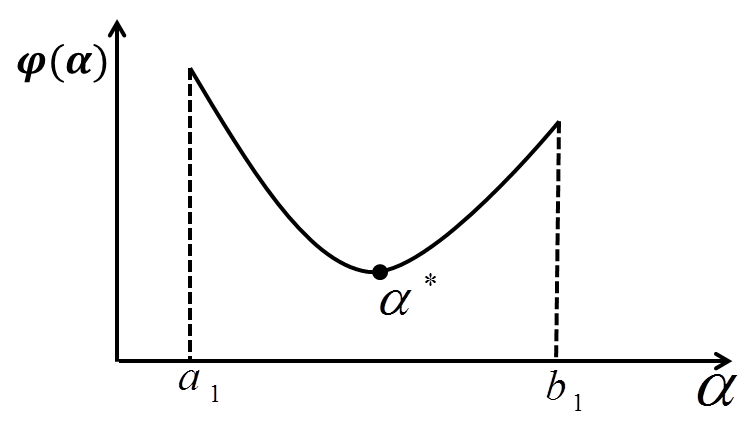
\includegraphics[height=3cm]{images/golden.jpg}
        \caption{黄金分割法示意图}
        \label{fig:黄金分割法示意图}
        \end{figure}
        % \textcolor[rgb]{1,0,0}{todo:图片:黄金分割法示意图}
        \par
        设$\varphi(\alpha)$是初始搜索区间$[a_1,b_1]$上的凸函数,如图(\ref{fig:黄金分割法示意图})所示。我们要不断收缩$[a_1,b_1]$以接近$\alpha ^*$(问:$[a_1,b_1]$如何确定)。设第$k$次分割的区间为$[a_k,b_k]$($\alpha^*\in [a_k,b_k]$)。取两个试操点$\lambda_k,\mu_k\in [a_k,b_k]$,且${\lambda}_k<{\mu}_k$,计算$\varphi({\lambda}_k)$和$\varphi({\mu}_k)$
        \par
        (1)若$\varphi({\lambda}_k) \le \varphi({\mu}_k)$则令$a_{k+1}={\alpha}_k,b_{k+1}={\mu}_k$,以形成$[{\alpha}_k,{\mu}_k]=a_{k+1},b_{k+1}$的新搜索空间;
        \par
        (2)若$\varphi({\lambda}_k) > \varphi({\mu}_k)$则令$a_{k+1}={\lambda}_k,b_{k+1}=b_k$,以形成$[{\lambda}_k,b_k]=a_{k+1},b_{k+1}$的新搜索空间。\\
        我们要求${\lambda}_k,{\mu}_k$满足以下条件:\par
        (1) $b_k-{\lambda}_k={\mu}_k-a_k$;\par
        (2) $b_{k+1}-a_{k+1}=\tau (b_k-a_k)$,其中,$\tau $为收缩率。\\
        由(1)(2)可知
        \begin{align*}
        {\lambda}_k & =a_k+(1-\tau)(b_k-a_k)\\
        {\mu}_k & =a_k+\tau(b_k-a_k)
        \end{align*}
        0.618法即$\tau=0.618$的分割方法。下面给出黄金分割法的步骤:\\
        \textbf{step1.}初始化。$[a_1,b_1],k=1$,精度要求$\epsilon>0$,$\tau=0.618$。\\
        \textbf{step2.}计算${\lambda}_1,{\mu}_1$。
        \begin{align*}
        {\lambda}_1 & =a_1+(1-\tau)(b_1-a_1)\\
        {\mu}_1 & =a_1+\tau(b_1-a_1)
        \end{align*}
        \textbf{step3.}确定新的搜索空间。\par
        3.1).计算$\varphi({\lambda}_k),\varphi({\mu}_k)$。\par
        3.2).若$\varphi({\lambda}_k) > \varphi({\mu}_k)$:\par
            \qquad \qquad 若$b_k-{\lambda}_k \le \epsilon$,则停止,得到${\mu}_k$;\par
            \qquad \qquad 否则,令$a_{k+1} := {\lambda}_k,b_{k+1} := b_k,{\lambda}_{k+1} := {\mu}_k$
            \begin{align*}
            \varphi({\lambda}_{k+1})=\varphi({\mu}_k),{\mu}_{k+1}:=a_{k+1}+0.618(b_{k+1}-a_{k+1})
            \end{align*}
        \par
        \qquad \qquad 计算$\varphi({\mu}_{k+1})$;\par
        \qquad \qquad 令$k=k+1$,返回step3.2)。\par
        \qquad 若$\varphi({\lambda}_{k}) \leqslant \varphi({\mu}_k)$:\par
            \qquad \qquad 若${\mu}_k-a_k \le \epsilon$,则停止,得到${\lambda}_k$;\par
            \qquad \qquad 否则,令$a_{k+1} := a_k,b_{k+1} := {\mu}_k,{\mu}_{k+1} := {\lambda}_k$
            \begin{align*}
            \varphi({\mu}_{k+1})=\varphi({\lambda}_k),{\lambda}_{k+1}:=a_{k+1}+0.382(b_{k+1}-a_{k+1})
            \end{align*}
            \par
            \qquad \qquad 计算$\varphi({\lambda}_{k+1})$;\par
            \qquad \qquad 令$k:=k=1$,返回step3.2)。\par
        前面,我们假设$\varphi (\alpha)$在$[a_,b_1]$上是某种凸函数,如果不是凸函数,则需要一定的改进,参考《最优化理论与方法》P72.袁亚湘,孙文瑜。
    \subsection{Fibonacci法}
        \par
        Fibonacci法与0.618法相近,区别在于它的收缩率$\tau$不是黄金分割数0.618,而是使用Fibonacci数。Fibonacci数列满足
        \begin{align*}
        &F_0  =F_1=1\\
        &F_{k+1}  =F_k+F_{k-1}\quad k=1,2,\dots
        \end{align*}
        令$\tau=\frac{F_{n-k}}{F_{n-k+1}}$,故
        \begin{align*}
        {\lambda}_k&=a_k+\left( 1-\frac{F_{n-k}}{F_{n-k+1}} \right) ({b}_k-a_k)\\
        &=a_k+\frac{F_{n-k-1}}{F_{n-k+1}}(b_k-a_k)\quad k=1,2,\ldots,n-1 \\
        {\mu}_k& =a_k+\frac{F_{n-k}}{F_{n-k+1}}(b_k-a_k) \quad k=1,2,\ldots,n-1
        \end{align*}
    \subsection{二次插值法}
        \subsubsection{插值简介}
            \par
            我们只知道$\varphi(\alpha)$的点列,如果我们假设$\varphi(\alpha)$是一个多项式函数(如二次函数),即用多项式来逼近$\varphi(\alpha)$,则称该方法为$\varphi(\alpha)$的插值方法。
            \par
            设$\varphi(\alpha)$的形式是一个二次多项式的形式,并将其设为
            \begin{align*}
            q(\alpha)=a{\alpha}^2+b{\alpha}+c
            \end{align*}
            其中:$a,b,c$为待定参数(待求参数)。3个参数要3个方程,而这3个方程的信息来自于已知$\varphi(\alpha)$点列。
            \par
            (1)如果我们仅给出1个点${\alpha}_1$,并且知道了$\varphi({\alpha}_1)$,${\varphi}'({\alpha}_1)$,${\varphi}''({\alpha}_1)$的值,则要求$q(\alpha)$在点${\alpha}_1$满足这3个值的情况。并称该方法为1点二次插值法,又称牛顿法。
            \par
            (2)如果我们给出2个点${\alpha}_1,{\alpha}_2$,并且知道了$\varphi({\alpha}_1)$,$\varphi({\alpha}_2)$,${\varphi}'({\alpha}_1)$或者$\varphi({\alpha}_1),{\varphi}'({\alpha}_1),{\varphi}'({\alpha}_2)$的值,则要求$q(\alpha)$在2点处满足相应的数值条件。称该方法为2点二次插值法又称割线法。
            \par
            (3)如果我们给出2个点${\alpha}_1,{\alpha}_2,{\alpha}_3$,并且知道了$\varphi({\alpha}_1),\varphi({\alpha}_2),\varphi({\alpha}_3),\ldots$称该方法为3点二次插值法又称割线法。
        \subsubsection{1点二次插值法(牛顿法)}
            \par
            设$q(\alpha)=a{\alpha}^2+b{\alpha}+c$,由
            \begin{align*}
            \left\{
            \begin{aligned}
            &{}q({\alpha}_1)=\varphi({\alpha}_1)\\
            &{}q'({\alpha}_1)=\varphi'({\alpha}_1)\\
            &{}q''({\alpha}_1)=\varphi''({\alpha}_1)
            \end{aligned}
            \right.
            \end{align*}
            可以求解$a,b,c$
            \begin{align*}
            \left\{
            \begin{aligned}
            &{}a=\varphi''{({\alpha}_1)/2}\\
            &{}b=\varphi'({\alpha}_1)-\varphi''({\alpha}_1){\alpha}_1
            \end{aligned}
            \right.
            \end{align*}
            则$q(\alpha)$的最小值为
            \begin{align*}
            {\alpha}_2:=-\frac {b}{2a}={\alpha}_1-\frac{\varphi'({\alpha}_1)}{\varphi''({\alpha}_1)}
            \end{align*}
            由此即得牛顿法的迭代公式:
            \begin{align*}
            {\alpha}_{k+1}={\alpha}_k-\frac{\varphi'({\alpha}_1)}{\varphi''({\alpha}_1)}
            \end{align*}
            注:这里的$k$并非$x_{k+1}=x_k+{\alpha}_k d_k$,而是$\alpha$的搜索序列。
            \par
            下面给出牛顿法的局部二阶收敛速度。假定$\varphi:R\to R,\varphi \in C^2,{\varphi}'({\alpha}^*) \ne 0 $,则当初始点${\alpha}_0$充分接近${\alpha}^*$时,由牛顿法迭代
            \begin{align*}
            {\alpha}_{k+1}={\alpha}_k-\frac{\varphi'({\alpha}_k)}{\varphi''({\alpha}_k)}\quad k=0,1,\ldots
            \end{align*}
            产生的点列$\{{\alpha}_k\}$收敛,即${\alpha}_k \to {\alpha}^*$。若$\varphi \in C^3$,则
            \begin{align*}
            \mathop {\lim} \limits_{k \to \infty}\frac {|{\alpha}_{k+1}-{\alpha}^*|}{|{\alpha}_{k}-{\alpha}^*|}=\bigg|\frac 12 \frac{\varphi'''({\alpha}^*)}{\varphi''({\alpha}^*)}\bigg|
            \end{align*}
            这表明
            \begin{align*}
            |{\alpha}_{k+1}-{\alpha}^*|=O(|{\alpha}_k-{\alpha}^{*}|^2)
            \end{align*}
        \subsubsection{2点二次插值法}
            \par
            \ding{172}设$q(\alpha)=a{\alpha}^2+b{\alpha}+c$,已知${\alpha}_1,{\alpha}_2$处的函数值$\varphi({\alpha}_1),\varphi({\alpha}_2),{\varphi}'({\alpha}_1)$,构建三元方程组,解$a,b,c$有
            \begin{align*}
            a&=\frac {{\varphi}_1-{\varphi}_2-{\varphi}_1'({\alpha}_1-{\alpha}_2)}{-{({\alpha}_1-{\alpha}_2)}^2}\\
            b&={\varphi}_1'+2 \frac{{\varphi}_1-{\varphi}_2-{\varphi}_1'({\alpha}_1-{\alpha}_2)}{{({\alpha}_1-{\alpha}_2)}^2} {\alpha}_1
            \end{align*}
            并且有
            \begin{align*}
            {\alpha}_3:={\alpha}_1-\frac{({\alpha}_1-{\alpha}_2){\varphi}_1'}{2[{\varphi}_1'-\frac {{\varphi}_1-{\varphi}_2}{{\alpha}_1-{\alpha}_2}]}
            \end{align*}
            写为迭代格式,有
            \begin{align*}
            {\alpha}_{k+1}={\alpha}_k-\frac{({\alpha}_k-{\alpha}_{k-1}){\varphi}_k'}{2[{\varphi}_k'-\frac {{\varphi}_k-{\varphi}_{k-1}}{{\alpha}_k-{\alpha}_{k-1}}]}
            \end{align*}
            \par
            \ding{173}设$q(\alpha)=a{\alpha}^2+b{\alpha}+c$,已知${\alpha}_1,{\alpha}_2$处的函数值$\varphi({\alpha}_1)$,${\varphi}'({\alpha}_1)$,${\varphi}'({\alpha}_2)$的,构建三元方程组,解$a,b,c$,有
            \begin{align*}
            {\alpha}_3:=-\frac {b}{2a}={\alpha}_1-\frac{{\alpha}_1-{\alpha}_2}{{\varphi}^{'}({\alpha}_1)-{\varphi}'({\alpha}_2)}{\varphi}'({\alpha}_1)
            \end{align*}
            写为迭代格式,有
            \begin{align*}
            {\alpha}_{k+1}={\alpha}_k-\frac{{\alpha}_k-{\alpha}_{k-1}}{{\varphi}'({\alpha}_k)-{\varphi}'({\alpha}_{k-1})}{\varphi}'({\alpha}_k)
            \end{align*}
            \par
            下面,我们给出二点二次插值法的收敛速度。设$\varphi(\alpha)$存在三阶连续导数,$\varphi(\alpha) \in C^3$,${\alpha}^*$满足${\varphi}'({\alpha}^*)=0,{\varphi}''({\alpha}^*) \ne 0$,则割线法迭代产生的序列$\{{\alpha}_k\}$收敛到$\{{\alpha}^*\}$,且其收敛速度的阶为$\frac{1+\sqrt{5}}{2} \approx 1.618$。\\
        \subsubsection{3点二次插值法}
            \par
            设$q(\alpha)=a{\alpha}^2+b{\alpha}+c$,已知${\alpha}_1,{\alpha}_2,\alpha_3$处的函数值$\varphi({\alpha}_1),\varphi({\alpha}_2),{\varphi}({\alpha}_3)$,构建三元方程组,解$a,b,c$有${\alpha}_4$
                    \begin{align*}
                    {\alpha}_4 &=\frac{1}{2}({\varphi}_1+{\varphi}_2)+\frac{1}{2}\frac {({\varphi}_1-{\varphi}_2)({\varphi}_2-{\varphi}_3)({\varphi}_3-{\varphi}_1)}{({\alpha}_2-{\alpha}_3){\varphi}_1+({\alpha}_3-{\alpha}_2){\varphi}_2+({\alpha}_1-{\alpha}_2){\varphi}_3}
                    \end{align*}
            上面的公式可以直接由\underline{拉格朗日插值公式}得到
                    \begin{align*}
                    L(\alpha) &=\frac{({\alpha}-{\alpha}_1)({\alpha}-{\alpha}_3)}{({\alpha}_1-{\alpha}_2)({\alpha}_1-{\alpha}_3)}{\varphi}_1+\frac {({\alpha}-{\alpha}_1)({\alpha}-{\alpha}_3)}{({\alpha}_2-{\alpha}_1)({\alpha}_2-{\alpha}_3)}{\varphi}_2 +\frac {({\alpha}-{\alpha}_1)({\alpha}-{\alpha}_2)}{({\alpha}_3-{\alpha}_1)({\alpha}_3-{\alpha}_1)}{\varphi}_3
                    \end{align*}
            令$L'(\alpha)=0$即可得到。
            \par
            下面讨论三点二次插值法的收敛速度。设$\varphi(\alpha)$存在四阶连续导数,$\varphi(\alpha) \in C^4$,${\varphi}'({\alpha}^*)=0,{\varphi}''({\alpha}^*) \ne 0$,则三点二次插值法产生的序列$\{{\alpha}_k\}$收敛速度约为$1.32$。\\
    \subsection{三次插值法}
        \par
        三次插值法使用一个三次四项式$q(\alpha)=c_1({\alpha}-a)^3+c_2({\alpha}-a)^2+c_3({\alpha}-a)+c_4$来逼近$\varphi(\alpha)$。这个$q(\alpha)$中的待定系数$\varphi$要有4个条件来确定,我们可以利用四点的函数值${\varphi}_1,{\varphi}_2,{\varphi}_3,,{\varphi}_4$,也可以利用三点函数值加一点的导数值${\varphi}_1,{\varphi}_2,{\varphi}_3,{\varphi}_4'$等等。三次插值法比二次插值法有较好的收敛效果。但通常要求计算导数组,且工作量比二次插值法大,所以,当导数容易求的时候,用三次插值法较好。
        \par
        上面讨论了基于区间收缩技术的黄金分割法和Fibonacci法,以及基于插值法的二次插值和三次插值法,并讨论了算法的收敛性。但上面讨论的都是精确一维搜索方法,求${\alpha}^*$往往需要很大的计算量。下面,我们介绍非精确的一维搜索方法:Armijo-Goldstein准则和Wolfe-Powell准则。
    \subsection{Armijo-Goldstein准则}
        \par
        Armijo(1966)和Goldstein(1965)分别提出不精确一维搜索过程,我们现在不要求${\alpha}^*$使$\varphi(\alpha)$最小。我们要求$\alpha$使得$\varphi(\alpha)<\varphi(0)$即可($\varphi(\alpha)=f(x_k+\alpha d_k)$)。设
                \begin{align*}
                J=\{\alpha > 0 \big|\varphi(\alpha)<\varphi(0)\}
                \end{align*}
        $J$是一个${\alpha}$的区间集合,则$J$中的点${\alpha}$是我们可以取值的。虽然$J$中的每一点皆是可取的,但我们这里要选择一个“恰当的”。为此,我们需要设置一些准则来约束$J$。如图(\ref{fig:Armijo准则示意图})所示
        \begin{figure}[H]
        \centering
        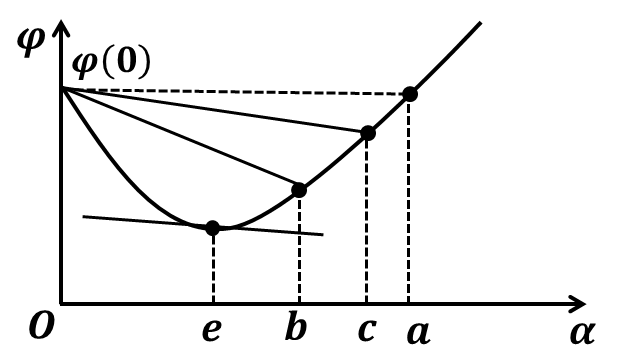
\includegraphics[height=3cm]{images/Armijo.jpg}
        \caption{Armijo准则示意图}
        \label{fig:Armijo准则示意图}
        \end{figure}
        % \textcolor[rgb]{1,0,0}{todo:图片:Armijo准则示意图}
        \par
        \ding{172}如图(\ref{fig:Armijo准则示意图})所示,$J=[0,a]$,为了保证目标函数单调下降,同时$\varphi$的下降不是太小(如果太小,可能导致序列$\{f(x_k)\}$的极限值不是极小值)。必须避免所选择的$\alpha$太靠近区间$J$的端点。我们要求
        \begin{align}\label{Armijo-Goldstein准则}
        \varphi({\alpha}_k) \leqslant \varphi(0)+\rho \varphi({\alpha}_k) {\varphi}'(0)
        \end{align}
        其中:$\rho \in (0,\frac 12)$。满足式(\ref{Armijo-Goldstein准则})的${\alpha}_k$指代的区间是$J_1=[0,c]$。
        \par
        \ding{173}为避免$\alpha$太小,我们加上另外一个要求
        \begin{align}\label{tab:2为避免下降太小}
        \varphi({\alpha}_k) > \varphi(0)+(1-\rho) \varphi({\alpha}_k){\varphi}'(0)
        \end{align}
        满足式(\ref{tab:2为避免下降太小})的多项式$J_2=[b,a]$。综合(\ref{Armijo-Goldstein准则})(\ref{tab:2为避免下降太小}),则有$J^*=[b,c]$,我们将(\ref{Armijo-Goldstein准则})(\ref{tab:2为避免下降太小})称为Armijo-Goldstein不精确线性搜索准则。一旦$\alpha \in J^*$,则称$\alpha $为可接受步长,$J^*$为可接受区间。
        \par
        \ding{174}如图\ref{fig:Armijo准则示意图}所示,A-G准则可能将$\alpha^*$排除在$J^*$之外。为此,Wolfe-Powell准则给出了一个更简单的条件来代替(\ref{tab:2为避免下降太小})
        \begin{align}\label{tab:3Wolfe-Powell准则}
        \varphi'({\alpha}_k) = \sigma {\varphi}'(0)> {\varphi}'(0)
        \end{align}
        解释为:可接受点$\alpha_k$处的斜率大于等于初始点斜率的$\sigma$倍。满足(\ref{tab:3Wolfe-Powell准则})的${\alpha}_k$构成区间为$J_3=[e,a]$。\\
        注:${\varphi}'(0)=g^\mathrm{T}_k d_k$。
        \par
        \ding{175}式(\ref{tab:3Wolfe-Powell准则})的不足在于,即使$\sigma \to \infty $时,也不能带来精确的线性搜索。但是,如果要求
        \begin{align}\label{tab:4Wolfe-Powell准则重约束}
        |{\varphi}'({\alpha}_k)| \leqslant \sigma |{\varphi}'(0)|
        \end{align}
        则可以满足。一般的,$\sigma$值越小,线性搜索越精确,满足(\ref{tab:4Wolfe-Powell准则重约束})的${\alpha}_k$的区间为$J_4$。
        \par
        综合(\ref{Armijo-Goldstein准则})(\ref{tab:3Wolfe-Powell准则}),则有$J^*=[e,c]$。我们称(\ref{Armijo-Goldstein准则})(\ref{tab:3Wolfe-Powell准则})为强Wolfe-Powell准则;称(\ref{Armijo-Goldstein准则})(\ref{tab:4Wolfe-Powell准则重约束})为$\alpha$强Wolfe-Powell准则。
        \par
        下面,我们给出Armijo-Goldstein不精确一维搜索方法的步骤:\\
        \textbf{step1.}初始化。在搜索区间$J^*=[0,a]$中取定初始点${\alpha}_0$,计算$\varphi(0),{\varphi}^{'}(0)$。给出$\rho \in (0,\frac 12),t \geqslant 1$,令$a_0:=0,b_0:=a,k:=0$。\\
        \textbf{step2.}检验准则(\ref{Armijo-Goldstein准则})。计算${\varphi}({\alpha}_k)$,若
                \begin{align*}
                \varphi({\alpha}_k) \leqslant \varphi(0)+\rho {\alpha}_k {\varphi}'(0)
                \end{align*}
                转到step3,否则,令${\alpha}_{k+1}:={\alpha}_k,b_{k+1}:={\alpha}_k$,转到step4。\\
        \textbf{step3.}检验准则(\ref{tab:2为避免下降太小}),若
                \begin{align*}
                \varphi({\alpha}_k) > \varphi(0)+(1-\rho) {\alpha}_k {\varphi}'(0)
                \end{align*}
                停止迭代,输出${\alpha}_k$;否则,令${\alpha}_{k+1}:={\alpha}_k,b_{k+1}:={\alpha}_k$,若$b_k < a$转到step4,否则,令${\alpha}_{k+1}:=t{\alpha}_k,k:=k+1$,转到step2。\\
        \textbf{step4.}取新的搜索点,取
                \begin{align*}
                {\alpha}_{k+1} = \frac {{\alpha}_{k+1}+ b_{k+1}}{2}
                \end{align*}
                令$k:=k+1$,转到step2。
        \par
        关于不精确以为搜索的收敛性,可以参考《最优化理论与方法》P102。\\
        总结:前面我们给出了求解$x_{k+1}=x_k+{\alpha}_k d_k$中${\alpha}_k$的精确线搜索方法:黄金分割法、Fibonacci 法、插值法以及非精确线搜索方法:A-G准则,W-P准则。后面,我们要给出求解方向$d_k$的方法。在此之前,我们给出MATLAB求一维无约束极值函数fminbnd的用法。
\section{MATLAB应用实例1}
    \par
    MATLAB中使用fminbnd函数命令来求解无约束一维极值优化,其调用格式为
    \par
    [x,fval,exitflag,output]=fminbnd(fun,$x_1$,$x_2$,options) \\
    其中:fun为目标函数,可以使句柄,可以是匿名函数也可以是函数文件;$x_1,x_2$为$x$的搜索区间;options为结构体;$x$为极小点;fval为极小值;exitflag返回函数fminbnd的求解状态:成功/失败;output返回fminbnd的求解信息:迭代次数、优化算法等。
    \par
    fminbnd函数的应用实例如下
    \begin{lstlisting}[language = Matlab]
    a = 9/7;
    fun = @(x) sin(x-a);
    x1 = 1;
    x2 = 2*pi;
    options = optionset('Display','iter');
    option.PlotFcns = @optimplotfval;
    [x,fval,exitflag,output] = fminbnd(fun,x1,x2,options)
    \end{lstlisting}
\section{搜索方向的确定}
    下面,将介绍一些求解方向$d_k$的方法。
    \subsection{最速下降法}
        \par
        最速下降法是以负梯度方向为搜索方向向量。设$f(x)$在$x_k$附近连续可微,且$g_k= \nabla f(x_k) \ne 0$,由泰勒公式展开
        \begin{align*}
        f(x) = f(x_k)+(x-x_k)^\mathrm{T} \nabla f(x_k)+ o (\|x-x_k\|)
        \end{align*}
        如果将$x$换为$x_k+\alpha d_k$,有
        \begin{align*}
        f(x_k+\alpha d_k)=f(x_k)+ \alpha g_k^\mathrm{T} d_k+o (\|\alpha d_k\|)
        \end{align*}
        则$f$在$x_k$处沿方向$d_k$的变化率为
        \begin{align*}
        \mathop {\lim}\limits_{\alpha \to 0} \frac {f(x_k+\alpha d_k)-f(x_k)}{\alpha}=g_k^\mathrm{T}  d_k
        \end{align*}
        由Gauchy-Schwartz不等式
        \begin{align*}
        |d^\mathrm{T}_k g_k| \leqslant \|d_k\|\ \|g_k\|
        \end{align*}
        所以,当且仅当$d_k=-g_k$时,$d^\mathrm{T}_k g_k$最小,从而有$-g_k$是最速下降方向。迭代格式为
        \begin{align*}
        x_{k+1} = x_k-{\alpha}_k g_k
        \end{align*}
        \par
        上面给出了$d_k=-g_k$,若对${\alpha}_k$采用精确线搜索,则有
        \begin{align*}
        \varphi(\alpha) \equiv  f(x_k+{\alpha}_k d_k)=\mathop {\min} \limits_{\alpha \geqslant 0}f(x_k+{\alpha} d_k)
        \end{align*}
        ${\alpha}_k$应满足${\varphi}'(\alpha) = \frac{\mathrm{d}}{\mathrm{d}\alpha}f(x_k+{\alpha} d_k)\big|_{\alpha = {\alpha}_k}= \nabla f(x_k+{\alpha}_k d_k)^\mathrm{T} d_k = 0$。由$d_k=-g_k= \nabla f(x_k)$有
        \begin{align*}
        g_{k+1}^\mathrm{T} g_k = d_{k+1}^\mathrm{T} d_k=0
        \end{align*}
        \par
        这表明,在相邻的两个迭代点$k,k+1$,函数$f(x)$的两个梯度方向是相互正交的,也就是迭代点列所走的路线是锯齿形的。当接近极小点时步长愈小,前进愈慢,至多有线性收敛速度。关于最速下降法的收敛性和收敛速度我们不再讨论。
    \subsection{牛顿法}
        \par
        牛顿法的基本思想是利用目标函数$f(x)$在收敛处的二次Taylor展开来逼近(代替)$f(x)$。求$x_{k+1}$使二次泰勒展开函数最小,以做为更新公式。
        \par
        假设$f(x)$是二次连续可微函数,$x_k \in R^n$,且Hesse矩阵$H \triangleq G(x) = {\nabla}^2 f(x)$是正定的。我们在$x_k$附近用二次泰勒展开近似$f$
        \begin{align*}
        f(x_{k}+s) \approx q^{(k)}(s) & = f(x_k)+\nabla f(x_k)^\mathrm{T} s+\frac 12 s^\mathrm{T} \nabla^2 f(x_k) s\\
        & =  f(x_k)+g_k^\mathrm{T} s+\frac 12 s^\mathrm{T}G_ks
        \end{align*}
        我们的目标是求$s$,使$q^{(k)}(s)$最小,求上式右边二次函数$q^{(k)}(s)$的稳定点
        \begin{align*}
        \nabla q^{(k)}(s) = g_k + G_k s=0
        \end{align*}
        有$s =-\frac {g_k}{G_k}$\footnote{这里要求$G_k$正定且非奇异}。其中:$s={\alpha}_k d_k$。如果我们令${\alpha}_k = 1$,就可得到更新公式(迭代公式)
        \begin{align*}
        x_{k+1} = x_k-\frac {g_k}{G_k}=x_k-G^{-1}_k g_k
        \end{align*}
        \par
        下面,给出牛顿法的局部收敛型和二阶收敛速度。设$f \in C^2(R)$,$x_k$充分靠近$x^*:\nabla f(x^*)=0$。如果${\nabla}^2 f(x)$正定,且Hesse矩阵$G(x)$满足Lipsditz条件\footnote{注:记Lipsditz条件为$Lip_r(D)$,其中,$r$为Lip常数,$x\in D$。},即$\exists L>0$,使得对$\forall i,j$,$\forall x,y \in R^n$,有
        \begin{align*}
        |G_{ij}(x)-G_{ij}(y)| \le L\|x-y\|
        \end{align*}
        其中:$G_{ij}(x)$是Hesse矩阵$G(x)$的$(i,j)$元素。则\underline{对一切$k$},牛顿迭代法所得到的的序列$\{x_k\}$收敛于$x^*$,并且有二阶收敛速度。
        \par
        在上述局部收敛性中,我们设$f$在$x^*$的Hessan矩阵是正定的,但这样并不是牛顿法收敛的必要条件。
        \par
        值得一提的是,当$x_0$远离$x^*$时,$G_k$不一定是正定的,因此牛顿方向不一定是下降方向,其收敛性不能保证。这说明恒取${\alpha}_k=1$的牛顿法是不合适的,所以我们用一维搜索方法来确定${\alpha}_k$,并且注意,仅当$\{{\alpha}_k\}$收敛到1时,牛顿法才是二阶收敛的,这时牛顿法的迭代公式为
        \begin{align*}
         & d_k  =-a^{-1}_k g_k\\
         & x_{k+1} =x_k+{\alpha}_k d_k
        \end{align*}
        称${\alpha}_k \ne 1$的方法为阻尼牛顿法。
        \par
        这里,我们给出阻尼牛顿法的算法流程\\
        \textbf{step1.}初始化。初始点$x_0 \in R^n$,终止误差$\varepsilon >0$,令$k:=0$。\\
        \textbf{step2.}计算$g_k$。若$\|g_k\| \leqslant \varepsilon $,终止迭代,输出$x_k$;否则转到step3。\\
        \textbf{step3.}求解$d_k$。解方程组构造牛顿方向,即解
        \begin{align*}
         a_k d = g_k
        \end{align*}
        \par
        求出$d_k$。\\
        \textbf{step4.}求${\alpha}_k$。进行一维线搜索,求${\alpha}_k$。\\
        \textbf{step5.}令$x_{k+1}=x_{k-1}+{\alpha}_k d_k,k:=k+1$,转到step2。
        \par
        下面,我们给出阻尼牛顿法的\underline{总体收敛性}:设$f:R^n \to R \in C^2(D)$,$D$为开凸集。如果$\forall x_0 \in D,\exists m >0$,使得$f(x)$在水平集$L(x_0)=\{x|f(x) \leqslant f(x_0)\}$上满足
        \begin{align*}
         u^\mathrm{T} \nabla^2 f(x)u \geqslant m \|u\|^2, \forall u \in R^n,x \in L(x_0)
        \end{align*}
        则在精确一维搜索下,带步长${\alpha}_k$的牛顿法产生的迭代序列$\{x_k\}$满足:\\
        (1) 当$\{x_k\}$为有穷点列时,$\exists k ,g(k)=0$;\\
        (2) 当$\{x_k\}$为无穷点列时,$\{x_k\}$收敛到$f$的唯一极小点$x^*$。
    \subsection{修正牛顿法}
        \par
        牛顿法面临的主要困难是Hesse矩阵$G_k$不一定是正定的,这时候二次搜索$q^k(s)$不一定有极小点$(q'=0,q'' > 0)$,甚至没有稳定点($q'=0$)。为了克服这个困难,Goldstein和Price(1967)提出了一种修正$G_k$的方法:当$G_k$非正定时,采用最速下降方向$-g_k$,将这种处理方法与\underline{角度准则结合},给出
        \begin{align*}
        d_k=\left\{
        \begin{aligned}
        &d_k^N \quad \cos \big< {d_k^N,-g_k} \big>\geqslant \eta\\
        &-g_k
        \end{aligned}
        \right.
        \end{align*}
        其中,$\eta >0$是正常数。这种方法能够保证$d_k$总满足
         \begin{align*}
          \cos \big< {d_k^N,-g_k} \big>\geqslant \eta
        \end{align*}
        从而算法的收敛性是可以保证的。
        \par
        Goldfold(1966)提出了一种修正方法,将Hesse矩阵$G_k$改为$G_k+V_k I$,其中,$V_k>0$,$G_k+V_k I$正定。较理想的$V_k$取值是:$V_k$不要远大于使$G_k+V I$正定的最小$V$。
        \par
        记$E_k=V_kI$,修正后的$G_k$为$\bar{G_k}$,下面给出修正牛顿法的算法程序:\\
        \textbf{step1.}初始化。初始搜索点$x_0 \in R^n$,容许误差$\varepsilon >0$,令$k:=0$。\\
        \textbf{step2.}计算$g_k$。若$\|g_k\| \leqslant \varepsilon $,终止迭代,输出$x_k$;否则转到step3。\\
        \textbf{step3.}计算$\bar{G_k}$。计算Hesse矩阵$G_k$,如果$G_k$正定,$V_k=0,\bar{G_k}=G_k+V_k I$;如果$G_k$非正定,给出$V_k$,$\bar{G_k}=G_k+V_k I$。\\
        \textbf{step4.}计算$d_k$。解$\bar{G_k}d=-g_k$,得到$d_k$。\\
        \textbf{step5.}计算${\alpha}_k$。\\
        \textbf{step6.}计算$x_{k+1}$。令$x_{k+1}=x_{k}+{\alpha}_k d_k,k:=k+1$,返回step2。
        \par
        上述算法的关键是如何解$\bar{G_k}$,也即如何解修正矩阵$E$。下面给出基于Cholesky分解的一种求$\bar{G_k}$的策略:先形成$G_k$的Cholesky分解${LDL}^\mathrm{T} $。然后令$\bar{G_k}=L\bar{D}L$。其中,$\bar{d}_{ii}=\max \{|d_{jj}|,\delta\}$,$d_{jj}$为$D$的对角元素,$\delta$为某个给定的小正数。但是,如果${G_k}$为对称不定矩阵,则其Cholesky分解可能不存在。另外,即使这种分解存在,其一般也是不稳定的,因为其矩阵分解的元素可能是无界的。进一步,当$G_k$仅微小波动时,$\bar{G_k}$也可能与$G_k$相差很大。
        \par
        为了克服Cholesky分解方法的不稳定性,Gill和Murray(1974)提出了一个数值稳定的处理方法。
        对称正定矩阵的Cholesky分解可以描述为
         \begin{align*}
          & d_{jj}=g_{jj}-{\mathop {\sum} \limits_{s=1}^{j-1} d_{ss}}-l_{js}^2\\
          & l_{ij}=\frac{1}{d_{jj}} \left( g_{ij}-{\mathop {\sum} \limits_{s=1}^{j-1} d_{ss}}-l_{js}l_{is} \right) , \quad i \geqslant {j+1}
        \end{align*}
        其中:$g_{ij}$表示$G_k$的元素,$d_{jj}$表示$D$的对角元素。
        \par
        现在,我们要求Cholesky分解因子$L$和$D$满足条件:\ding{172}$D$的所有元素是严格正的;\ding{173}$L,D$的所有元素满足一致有界,也就是说,对$k=1,2,\dots,n$和某一个正数$\beta$,要求
         \begin{align}\label{tab:Cholesky分解的要求}
          & d_{kk}> \delta  \notag \\
          & |r_{ik}| \leqslant \beta \quad i>k
        \end{align}
        其中:$r_{ik}=l_{ik}\sqrt{d_{kk}}$,$\delta$为某个给定的小正数。
        \par
        下面,我们来描述一下这个分解的第$j$步,假设修改Cholesky分解的前$j-1$列已经计算出来,对于$k=1,2,\ldots,j-1$,式(\ref{tab:Cholesky分解的要求})成立。先计算
         \begin{align*}
        {r_j}=\left|{\xi}_j-{\mathop {\sum} \limits_{s=1}^{j-1} d_{ss}l_{js}^2}\right|
        \end{align*}
        其中:${\xi}_j$取$g_{jj}$,试验值$\bar{d}=\max{r_j,\delta}$。\par
        为了断定$\bar{d}$是否可以接受作为$D$的第$j$个元素。我们检验$r_{ij}=l_{ij}\sqrt{\bar{d}}$是否满足式(\ref{tab:Cholesky分解的要求})。并且由$l_{ij}=r_{ik}/\sqrt{d_{jj}}$得到$L$的第$j$列,否则
         \begin{align*}
        d_{jj}=\left|{\xi}_j-{\mathop {\sum} \limits_{s=1}^{j-1} d_{ss}l_{js}^2}\right|
        \end{align*}
        其中:${\xi}_j=g_{jj}+e_{jj}$。选取正数$e_{jj}$使得$\max |r_{ij}|=\beta$,并且也产生$L$的第$j$列。
        \par
        上述过程完成时,我们得到了正定矩阵$\bar{G_k}$的Cholesky分解
         \begin{align*}
        \bar{G_k}={LDL}^\mathrm{T} =G_k+E
        \end{align*}
        其中:$E$是非负对角矩阵,对角元素为$e_{jj}$。对于给定的$G_k$,这个非负对角矩阵$E$依赖于$\beta$,Gill和Murray证明:如果$n>1$,则
        \begin{align*}
        \|E(\beta)\|_\infty <(\frac{\xi}{\beta}+(n-1)\beta)^2+2(r+(n-1){\beta}^2)+\delta
        \end{align*}
        其中:$\xi$是$G_k$的非对角元素的最大模,$r$是$G_k$的对角元素的最大模。
    \subsection{信赖域方法}
        在目标函数$f$的\underline{鞍点}处,我们有时会遇到$\nabla f(x_k)=0$,$\nabla^2 f(x_k)$非半定这种特殊情形。此时,前面的修正牛顿法就不好用了。一种解决策略是用函数的负曲率方向作为搜索方向。保证目标函数值仍是下降的。
        \par
        前面介绍的牛顿法的基本思想是在$x_k$附近用二次函数
        \begin{align*}
        q^{(k)}(s) = f(x_k)+g_k^\mathrm{T}  s+\frac 12 s^\mathrm{T}  G_k s
        \end{align*}
        来逼近$f(x)$,并以$q^{(k)}(s)$的极小点$s_k$修正$x_k$,反复迭代。其迭代公式为
        \begin{align*}
        x_{k+1} =x_k+s_k
        \end{align*}
        牛顿法显然具有二阶收敛速度,但其仅具有局部收敛性,即只有当$s$充分小时,$q^{(k)}(s)$才能逼近$f(x)$。我们后面说的阻尼牛顿法具有总体收敛性。下面,我们将介绍一种新的方法 - 信赖域法。这种方法不仅具有总体收敛性,并且也可以解决Hesse矩阵$G_k$非正定及$x_k$为鞍点等困难。
        \par
        在给定一个点$x_k$后,我们先定义一个步长上界$h_k$,并且由此给出$x_k$的一个邻域${\Omega}_k$
         \begin{align*}
        {\Omega}_k =\{x|\ \|x-x_k\| \leqslant h_k\}
        \end{align*}
        ${\Omega}_k$称为信赖域。我们假设在${\Omega}_k$中用$q^k(s)$来逼近$f(x)$是恰当的,然后求搜索方向$s_k$,使$q^k(s)$最小,即
         \begin{align*}
        & \mathop {\min} \limits_s \ q^k (s)=f(x_k)+g^\mathrm{T} _k s+\frac 12 s^\mathrm{T} G_ks \\
        & s.t.\quad  \|s\| \leqslant h_k
        \end{align*}
        其中:$h_k$是步长上界,$s = \|x-x_k\|$,范数$\| \cdot \|$可以用$L^2$范数$L_\infty$范数。
        \par
        值得一提的是,$G_k$为Hesse矩阵,如果难于计算,可采用后面介绍的方法做近似。假设我们给出了$h_k$,我们来尝试给出$\| \cdot \|=\|\cdot\|_2$情况的解。如果取$\| \cdot \|$为$L^2$范数,则相应的模型变为
        \begin{align*}
        & \mathop {\min} \limits_s \ q^k (s)=f(x_k)+g^\mathrm{T} _k s+\frac 12 s^\mathrm{T} G_ks \\
        & s.t. \quad s^\mathrm{T} s \leqslant h_k^2
        \end{align*}
        \par
        \ding{172}如果$s^*$在$s^\mathrm{T} s \leqslant h_k^2$内,则约束不起作用,所以只需要求解
         \begin{align*}
         \mathop {\min} \limits_s \  q^k (s)=f(x_k)+g^\mathrm{T} _k s+\frac 12 s^\mathrm{T} G_ks
        \end{align*}
        即可。那么就变为牛顿法:当$G_k$为正定时,$s_k=-G_k^{-1}g_k$为解。
        \par
        \ding{173}如果$s^*$在边界上有$s^\mathrm{T} s=h_k^2$,则引进Lagrange函数。
        \begin{align*}
        L(s,\lambda ) = q^{(k)}(s) + \frac 12 \lambda (s^\mathrm{T} s - h_k^2)
        \end{align*}
        \par
        上面,我们假设假设我们已经给出了$h_k$,那么,我们该如何求$h_k$?一般地,当$q^{(k)}(s)$与$f(x_b+s)$之间的一致性满足某种要求时,应选取尽可能大的$h_k$。设$\Delta f_k$是$f$在第$k$步的实际下降量。
        \begin{align*}
         \Delta f_k = f_k - f (x_k + s_k)
        \end{align*}
        对应的$q^{(k)}(s)$下降量为
         \begin{align*}
         \Delta q^{(k)} = f_k - q^{(k)}(s)
        \end{align*}
        定义二者比值
        \begin{align*}
         r_k = \Delta f_k / \Delta q^{(k)}
        \end{align*}
        $r_k$衡量了$q^{(k)}(s_k)$与目标$f(x_k+s_k)$的近似程度,$r_k$越接近1,表明近似程度越高。下面给出信赖域方法的算法程序:\\
        \textbf{step1.}初始化。$x_0 \in R^n,h_0=\|g_0\|,\mu = \frac 14, \eta = \frac 34 ,\varepsilon >0,k:=1$。\\
        \textbf{step2.}给出$x_k \in R^n,h_k \in R$,计算$g_k$。若$\|g_k\| \leqslant \varepsilon $,终止迭代,输出$x_k$;否则,计算$G_k$。\\
        \textbf{step3.}解信赖域模型,求出$s_k$。\\
        \textbf{step4.}求$f(x_k+s_k)$和$r_k$的值。\\
        \textbf{step5.}如果$r_k \leqslant  \mu $,令$h_{k+1} = \|s_k\|/4$;
        如果$r_k > \eta $并且$\|s_k\| = h_k$,令$h_{k+1}=2h_k$;
        否则,令$h_{k+1}=h_k$。\\
        \textbf{step6.}如果$r_k \leqslant 0 $,令$x_{k+1} = x_k$,否则$x_{k+1}=x_k+s_k$。令$k:=k+1$,返回step2。
        \par
        下面,给出信赖域的总体收敛性和收敛速度。
        \par
        (1)设$B \subset R^n$是有界集,$x_k \in B,\forall N$,若$f \in C^2$在有界集$B$上$\|G_k\|_2 \leqslant N,M \geqslant 0$,则信赖域算法产生一个满足一阶二阶必要条件的聚点$x^{\infty }$
        \par
        (2)若零点$x^{\infty }$还满足$f$的Hesse矩阵$G^{\infty}$是正定的,那么,对于主序列,有$r_k \rightarrow 1,x_k \to x^{\infty},g(b(x_k))>0$,以及充分大的$k$,约束$\|s\|_2 < h_k$,此外收敛速度是二阶的。
    \subsection{共轭梯度法}
        \par
        共轭方向法是介于最速下降法和牛顿法之间的一个方法,它仅需要一阶导数信息,但克服了最速下降法收敛速度慢的特点,又避免了牛顿法计算存贮二阶导数信息的麻烦。典型的共轭方向法有共轭梯度法和拟牛顿法。我们先来介绍共轭方向法。
        \par
        设$G \in R^{n \times n}$是对称正定矩阵,$d_1,d_2$是$n$维非零向量。如果$d_1^\mathrm{T}  G d_2 = 0$,则称向量$d_1,d_2$是$G$共轭的。类似地,设$d_1,d_2,\dots,d_m$是$R^n$中一组非零向量。如果$\forall ij,i \neq j$有$d_i^\mathrm{T} G d_j=0$,则称$d_1,d_2,\dots,d_m$是$G$-共轭的。
        \par
        显然,如果$d_1,d_2,\ldots,d_m$是$G$-共轭的,那么它们是线性无关的。下面给出共轭方向法的算法流程(共轭方向法即方向$d_k$共轭)。\\
        \textbf{step1.}初始化。$x_0\in R^n$,计算$g_0 = g(x_0)$,给一个$d_0$使$d_0^\mathrm{T}  g_0 <0$,令 $k:=0$。\\
        \textbf{step2.}计算${\alpha}_k,x_{k+1}$,$\mathop {\min} \limits_{\alpha \in R}f(x_k+\alpha d_k)$。若$
        \nabla f(x^{k+1})=0$或$k=n-1$,则算法停止;否则转到step3。\\
        \textbf{step3.}计算$d_{k+1}$,使$d_{k+1}^\mathrm{T}  G d_j=0,j=0,1,\ldots ,k$(共轭方向法),$d_k \in R^n$。\\
        \textbf{step4.}令$k:=k+1$转到step2。
        \begin{lemma}[扩张子空间定理]
        给定严格凸的二次正定函数
        \begin{align*}
         f(x)=\frac 12 x^\mathrm{T} Gx+b^\mathrm{T} x+c
        \end{align*}
        其中:$G=G^\mathrm{T} \succ 0$。若$\{d_0,d_1,\ldots,d_{n-1}\}$是$G$-共轭向量,则$\forall x_0\in R^n$,共轭方向法至多经过$n$步的精确线搜索后,可以找到$f(x)$的最小点。特别地,对$i=0,1,\ldots.$迭代点$x_{i+1}$都是$f(x)$在$x_0$和方向$d_0,d_1,\ldots,d_i$所张成的线性流形(仿射子空间)$\mathcal{M}$中的最小点。
        \begin{align*}
         \mathcal{M}(x_0;s_i) \equiv \mathcal{M}(x^0;\{ d_0,d_1,\ldots,d_i\})=\left\{x \Big|x=x_0+\mathop {\sum} \limits_{j=0}^i{\lambda}_jd_j,{\lambda}_j \in R\right\}
        \end{align*}
        其中:用$s_i=span\{d_0,d_1,\ldots,d_i\}$表示基向量$d_0,d_1,\ldots,d_i$张成的线性子空间,简记作$\mathcal{M}_i$。
        \end{lemma}
        \subsubsection{共轭梯度的引出}
            \par
            1952,Hestenes和Stiefel在求解线性方程组时,提出共轭梯度法(线性方程组等价于极小化一个正定二次函数)。1964年,Fletcher和Reeves提出了无约束极小问题的共轭梯度法,共轭梯度法就是使得最速下降方向$g_k$具有共轭性。下面,我们以正定二次函数为例来推导共轭梯度法。设:
            \begin{align*}
            f(x)=\frac 12 x^\mathrm{T} Gx+b^\mathrm{T} x+c
            \end{align*}
            $f$的梯度为
            \begin{align*}
            g(x)=Gx+b
            \end{align*}
            我们令
            \begin{align*}
            d_0=-g_0
            \end{align*}
            则$x_1=x_0+{\alpha}_0d_0$。由精确线搜索性质
            \begin{align*}
            g_1^\mathrm{T} d_0=0
            \end{align*}
            令
            \begin{align}
            \label{eq1}
            d_1=-g_1+{\beta}_0d_0
            \end{align}
            选择${\beta}_0$,使得
            \begin{align*}
            d_1^\mathrm{T} Gd_0=0
            \end{align*}
            对(\ref{eq1})两边同乘以$d_0^\mathrm{T} G$,有
            \begin{align*}
            {\beta}_0 = \frac {g_1^\mathrm{T} Gd_0}{d_0^\mathrm{T} Gd_0}= \frac {g_1^\mathrm{T} (g_1-g_0)}{d_0^\mathrm{T} (g_1-g_0)}= \frac {g_1^\mathrm{T} g_1}{g_0^\mathrm{T} g_0}
            \end{align*}
            由扩张子空间引理,$g_2^\mathrm{T} d_2=0,i=0,1$,利用$d_0=-g_0,d_1=-g_1+{\beta}_0d_0$,可知
            \begin{align*}
            g_2^\mathrm{T} g_0=0\quad g_2^\mathrm{T} g_1=0
            \end{align*}
            又令
            \begin{align*}
            d_2=-g_2+{\beta}_0d_0+{\beta}_1d_1
            \end{align*}
            选择${\beta}_0$和${\beta}_1 $,使得$d_2^\mathrm{T} Gd_2=0,i=0,1,\ldots$,从而有
            \begin{align*}
            &{\beta}_0=0\\
            &{\beta}_1=\frac {g_2^\mathrm{T} (g_2-g_1)}{d_1^\mathrm{T} (g_2-g_1)}= \frac {g_2^\mathrm{T} g_2}{g_1^\mathrm{T} g_2}
            \end{align*}
            一般的,在第$k$次迭代中,令
            \begin{align}
            \label{eq2}
            d_k=-g_k+\mathop {\sum} \limits_{i=0}^{k-1}{\beta}_id_i
            \end{align}
            选择${\beta}_i$,使$d_k^\mathrm{T} Gd_i=0,i=0,1,\ldots,k-1$。已假定
            \begin{align}
            \label{eq3}
            g_k^\mathrm{T} d_i=0,g_k^\mathrm{T} g_i=0,i=0,1,\ldots,k-1
            \end{align}
            对(\ref{eq2})式和$d_j^\mathrm{T} G,j=0,1,\ldots,k-1$,则
            \begin{align*}
            {\beta}_j=\frac {g_k^\mathrm{T} Gd_j}{d_j^\mathrm{T} Gd_j}= \frac {g_k^\mathrm{T} (g_{j+1}-g_j)}{d_j^\mathrm{T} (g_{j+1}-g_j)}\quad j=0,1,\ldots,k-1
            \end{align*}
            由式(\ref{eq3}),有
            \begin{align*}
            &g_k^\mathrm{T} g_{j+1}=0\quad j=0,1,\ldots,k-2\\
            &g_k^\mathrm{T} g_{j}=0\quad j=0,1,\ldots,k-1
            \end{align*}
            故得${\beta}_j=0,j=0,1,\ldots,k-2$,和
            \begin{align*}
            {\beta}_{k-1}=\frac {g_k^\mathrm{T} (g_{k}-g_{k-1})}{d_{k-1}^\mathrm{T} (g_{k}-g_{k-1})}= \frac {g_k^\mathrm{T} g_k}{g_{k -1}^\mathrm{T} g_{k -1}}
            \end{align*}
            因此,共轭梯度法的公式为
            \begin{align*}
            &x_{k+1}=x_k+{\alpha}_kd_k\\
            &d_{k+1}=-g_{k+1}+{\beta}_kd_k\\
            &k = 0,1,\ldots
            \end{align*}
            其中:$d_0=-g_0$,${\alpha}_k$由线搜索得到,${\beta}_k$有以下几种计算公式:
            \begin{align*}
            & {\beta}_{k}=\frac {g_{k+1}^\mathrm{T} g_{k+1}}{g_k^\mathrm{T} g_{k}}   \tag*{[Fletcher-Reeves公式]}\\
            & {\beta}_{k}=\frac {g_{k+1}^\mathrm{T} (g_{k+1}-g_k)}{g_k^\mathrm{T} g_{k}}  \tag*{[Polak-Ribion-Polyak公式]}\\
            & {\beta}_{k}=\frac {g_{k+1}^\mathrm{T} (g_{k+1}-g_k)}{d_k^\mathrm{T} (g_{k+1}-g_k)}  \tag*{[Growder-Wolfe公式]}\\
            & {\beta}_{k}=\frac {g_{k+1}^\mathrm{T} G_{k+1}d_k}{d_k^\mathrm{T} G_{k+1}d_{k}}  \tag*{[Doniel公式]}\\
            & {\beta}_{k}=-\frac {g_{k+1}^\mathrm{T} g_{k+1}}{d_k^\mathrm{T} g_{k}} \tag*{[Dixon公式]}\\
            & {\beta}_{k}=\frac {g_{k+1}^\mathrm{T} g_{k+1}}{d_k^\mathrm{T} (g_{k+1}-g_k)} \tag*{[Dai-Yuan公式]}
            \end{align*}
            对上面的${\beta}_{k}$计算公式,如果${\alpha}_{k}$采用精确线搜索,那么$g_{k+1}^\mathrm{T} d_k=0$。特别地,当$g_{k+1} \neq 0$时,有
            \begin{align*}
            g_{k+1}^\mathrm{T} d_{k+1}=-\|g_{k+1}\|^2 < 0
            \end{align*}
            此时,搜索方向$d_{k+1}$一定是目标函数下降方向。在实际应用中,Fletcher-Reeves公式较为普通,对于一些大型的优化问题,Polak-Ribion-Polyak公式的结果较好。下面讨论共轭梯度法的收敛性。
            \par
            由于共轭梯度法的计算公式较多,我们仅给出精确线搜索下FR共轭梯度的总体收敛性。设$f:R^n \to R$在有界水平集$L=\{x \in R^n |f(x) \leqslant f(x_0)\}$上连续可微,即$f \in C'(L)$。那么,精确线搜索下的FR共轭梯度法,产生的序列$\{x_k\}$至少有一个聚点是驻点,即\par
            (1)当$\{x_R\}$是有穷点列时,最后一个点$x^*$是$f$的驻点。\par
            (2)当$\{x_R\}$是无穷点列时,它必有极限点,且其任意极限点为$f$的驻点。\par
            共轭梯度法具有二次终止性,即对于二次函数,采用精确一维搜索的共轭梯度法在$n$次迭代后终止。此外,共轭梯度法是至少线性收敛的,且在适当条件下,共轭梯度法具有$n$步二阶收敛性。
    \subsection{拟牛顿法}
        \par
        牛顿法具有较快的收敛速度,关键是利用了Hesse矩阵提供的曲率信息,但是计算Hesse矩阵困难且其存储量极大。拟牛顿法利用目标函数$f$和一阶导数$g$来构造Hesse矩阵的近似。由此获得一个搜索方向,生成新的迭代点。采用不同的Hesse矩阵近似,对应着不同的拟牛顿法。
        \par
        设$f:R^n \to R$在开集$D \subset R^n$上的二次函数连续可微函数$f \in C^2(D)$,假设我们已经知道了$x_{k+1} \in R^n$的具体值,$f$在$x_{k+1}$附近的二次函数近似为
        \begin{align*}
         f(x) \approx f(x_{k+1})+g_{k+1}^\mathrm{T} (x-x_{k+1})+\frac 12 (x-x_{k+1})^\mathrm{T} G_{k+1}(x-x_{k+1})
        \end{align*}
        上式两边对$x$求导,有
        \begin{align}
         \label{eq求导}
         g(x) \approx g_{k+1} + G_{k+1}(x-x_{k+1})
        \end{align}
        \ding{172}如果$G_{k+1}$已知,且令$g(x) \equiv g(x_{k+2}) \approx 0$,则由上式(\ref{eq求导})可得到牛顿法的迭代公式
         \begin{align*}
         x_{k+2}=x_{k+1}-G_{k+1}^{-1}g_{k+1}
        \end{align*}
        \ding{173}如果$G_{k+1}$未知,如何由式(\ref{eq求导})求$x_{k+2}$呢?
        \par
        令$x=x_k,s_k=x_{k+1}-x_k,y_k=g_{k+1}-g_k$,得
         \begin{align*}
         G_{k+1}^{-1}y_k \approx s_k
        \end{align*}
        显然,对于二次函数$f$,上式是精确成立的。如果我们构造Hesse矩阵的$G_{k+1}$的近似,我们要求其近似能够满足上述等式,即
         \begin{align*}
         H_{k+1} y_k = s_k
        \end{align*}
        其中:$H_{k+1}$是$G_{k+1}^{-1} $的近似。或者设$B_{k+1}$是$G_{k+1}$的近似,则
         \begin{align*}
         B_{k+1} s_k = y_k
        \end{align*}
        我们把$B_{k+1}$或者$H_{k+1}$满足的等式称作拟牛顿条件或者拟牛顿方程。
        \par
        一般的拟牛顿算法流程如下:\\
        \textbf{step1.}初始化。$x_0 \in R^n,H_0 \in R^{n \times n},0 \leqslant \varepsilon <1,k:=0$。\\
        \textbf{step2.}如果$\|g_k\| \leqslant \varepsilon$,输出$x_k$;否则计算$d_k=-H_kg_k$。\\
        \textbf{step3.}求$\alpha_k$。计算$\arg \mathop {\min}\limits_{\alpha}f(x_k+d_k \alpha)$,令$x_{k+1}=x_k+{\alpha}_kd_k$。\\
        \textbf{step4.}校正$H_k$产生$H_{k+1}$。其中$H_{k+1}$要使得$H_{k+1}y_k=s_k$成立
        \begin{align*}
         y_k =g_{k+1} - g_k\\
         s_k =x_{k+1} - x_k
        \end{align*}
        \textbf{step5.}$k:=k+1$,转step2.
        \par
        在上述拟牛顿算法中,$H_0$通常取单位矩阵$H_0=I$。由于在每一次迭代中不定矩阵$H_k$总是不断变化的,故拟牛顿法也称为变尺度方法。

        上面介绍了拟牛顿法的思想及拟牛顿法的算法流程。下面给出$H_k$的一些计算公式。
        \subsubsection{对称秩1校正公式}
            \par
            假设$H_k$已知,在构造满足$H_{k+1}y_k=s_k$的矩阵$H_{k+1}$时,可以令
            \begin{align*}
            H_{k+1} =H_{k} +E_k
            \end{align*}
            其中:$E_k$是一个低秩的校正矩阵。秩1校正是指
            \begin{align*}
            E_{k} = uv^\mathrm{T}
            \end{align*}
            即$H_{k+1}=H_k+uv^\mathrm{T} $。由拟牛顿条件,有
            \begin{align*}
            &H_{k+1}y_k=(H_k+uv^\mathrm{T} )y_k=s_k\\
            \Rightarrow \quad &(v^\mathrm{T} y_k)u=s_k-H_ky_k
            \end{align*}
            故$u$必定是在方向$s_k-H_ky_k$上。假设$s_k-H_ky_k \neq 0$(否则,$H_k$已满足拟牛顿条件)。向量$v$满足$v^\mathrm{T} y \neq 0$,则
            \begin{align}
            \label{eq对称秩1校正1}
            H_{k+1}y_k=H_k+\frac {1}{{v}^\mathrm{T} y_k}(s_k-H_ky_k)v^\mathrm{T}
            \end{align}
            由于Hesse矩阵是对称的,故要求Hesse逆近似也是对称的,从而取$v=s_k-H_ky_k$,得
            \begin{align}
            \label{eq对称秩1校正2}
            H_{k+1}y_k=H_k+\frac {(s_k-H_ky_k)(s_k-H_ky_k)^\mathrm{T} }{(s_k-H_ky_k)^\mathrm{T} y_k}
            \end{align}
            式(\ref{eq对称秩1校正1})称为Broyden秩一校正公式。特别地,当$v=y_k$时,称为Broyden秩一校正公式。
        \subsubsection{对称秩2校正公式}
            SR1校正不能保证$H_k$的正定性,仅当$(s_k-H_ky_k^\mathrm{T} )y_k>0$时,SR1校正才具有正定性,而这个条件往往很难保证。设对称秩二校正为
            \begin{align*}
             H_{k+1} = H_k+auu^\mathrm{T} +bvv^\mathrm{T}
            \end{align*}
            令$H_{k+1}$满足拟牛顿条件,则
            \begin{align*}
             H_{k}y_k +auu^\mathrm{T} y_k+bvv^\mathrm{T} y_k=s_k
            \end{align*}
            这里$u$和$v$并不唯一确定,但$u$和$v$的明显选择是
            \begin{align*}
             u=s_k\quad v=H_ky_k
            \end{align*}
            于是
            \begin{align*}
             au^\mathrm{T} y_k=1\quad bv^\mathrm{T} y_k=-1
            \end{align*}
            确定出
            \begin{align*}
             & a=1/{u^\mathrm{T} y_k}=1/{s_k^\mathrm{T} y_k}\\
             & b=-1/{v^\mathrm{T} y_k}=-1/{y_k^\mathrm{T} H_ky_k}
            \end{align*}
            因此
            \begin{align}
            \label{eq4}
             H_{k+1}=H_k+\frac {s_ks_k^\mathrm{T} }{s_k^\mathrm{T} y_k}-\frac {H_ky_ky_k^\mathrm{T} H_k}{y_k^\mathrm{T} H_ky_k}
            \end{align}
            (\ref{eq4})式称为DFP公式,它是由Davidon(1959)提出,后来由Fletder和Powell(1963)发展的。DFP校正能保证$H_k$的正定性,每次迭代需要$3n^2+O(n)$次乘法运算,且方法具有超线性收敛速度。但DFP方法具有数值不稳定性,有时产生数值上奇异的Hessen矩阵。
        \subsubsection{BFGS校正公式}
            类似于关于$H_k$我们得到的DFP修正公式。那样,我们也可以从$B_k$得到BFGS修正公式
            \begin{align*}
             & B_{k+1}^{(BFGS)}=B_k+\frac {y_ky_k^\mathrm{T} }{y_k^\mathrm{T} s_k}-\frac {B_ks_ks_k^\mathrm{T} B_k}{s_k^\mathrm{T} B_ks_k}
            \end{align*}
            由于$B_ks_k=-{\alpha}_kg_k,B_kd_k=-g_k$,故上式也可以写为
            \begin{align*}
             & B_{k+1}^{(BFGS)}=B_k+\frac {g_kg_k^\mathrm{T} }{g_k^\mathrm{T} d_k}-\frac {y_ky_k^\mathrm{T} }{{\alpha}y_k^\mathrm{T} d_k}
            \end{align*}
            事实上,只要通过对DFP校正公式作简单的变换,$H \leftrightarrow B,s \leftrightarrow y$,就可以得到$B_k$的BFGS校正公式。对$B_k$的BFGS应用两次逆的秩一校正的Sherman—Morrison公式,就可以得到$H_k$的BFGS校正公式
            \begin{align*}
             & H_{k+1}^{(BFGS)}=\left( I-\frac {s_ky_k^\mathrm{T} }{s_k^\mathrm{T} y_k} \right) H_k \left( I-\frac {y_ks_k^\mathrm{T} }{s_k^\mathrm{T} y_k} \right)  +\frac {s_ks_k^\mathrm{T} }{s_k^\mathrm{T} y_k}
            \end{align*}
            BFGS是非常好的拟牛顿公式,它具有DFP校正所具有的性质,并且当采用不精确线搜索时,BFGS还具有总体收敛性质。
    \subsection{模式搜索法:不使用导数的最优化方法}
        \par
        前面介绍了基于导数的最优化方法:最速下降法、牛顿法、修正牛顿法、信赖域方法、共轭梯度法、拟牛顿方法,这些方法都是当目标函数$f$的导数易求时,才能较好的使用,但如果函数$f$不规则,我们又该如何处理?下面,我们来介绍一些不使用导数的最优化方法:模式搜索法、Rosenbrock方法和Powell方法。
        \par
        1961年,Hooke和Jeeves设计了模式搜索方法,算法从初始基点开始,包括两种类型的移动。\ding{172}探测移动:依次沿着$n$个坐标轴进行,用以确定新的基点和利于函数值下降的方向。\ding{173}模式移动:沿相邻两个基点连线方向进行,试图顺着“山谷”使函数值更快的减小。
        \par
        设$x \in R^n$,$f:R^n \rightarrow R$,坐标方向为$e_j,j=1,2,\ldots,n$。
        \begin{align*}
         e_j=(0,0,\ldots,0,\overset{j}{1},0,\ldots,0)^\mathrm{T}
        \end{align*}
        给定初始步长$\delta$和加速因子$\alpha$,使任取初始点$x_1$作为第1个基点,$x_j$为第$j$个基点,在每轮探测移动中,自变量$x$用$y_j$表示,即$y_j$是沿着$e_j$探测的出发点,$y_1$是沿$e_1$探测的出发点,$y_{n+1}$是沿$e_{n}$探测得到的点。
        \par
        首先,从$y_1=x$出发,进行探测移动。先沿$e_1$探测,如果$f(y_1+\delta e_1)<f(y_1)$则探测成功,令$y_2=y_1+\delta e_1$,并从$y_2$出发,沿$e_2$进行探测;否则,沿$e_1$方向探测失败,再沿$-e_1$方向探测。
        如果$f(y_1-\delta e_1)<f(y_1)$则探测成功,令$y_2=y_1-\delta e_1$,并从$y_2$出发,沿$e_2$进行探测。
        如果$f(y_1-\delta e_1) \geqslant f(y_1)$则沿$-e_1$探测失败,令$y_2=y_1$,再从$y_2$出发,沿$e_2$进行探测。方法同上,得到的点记作$y_3$,直到$y_{n+1}$终止。
        如果$f(y_{n+1}) < f(x_1)$则$y_{n+1}$作为新的基点,$x_2:=y_{n+1}$。这时,$d=x_2-x_1$是利用函数值减小的方向。
        \par
        然后,沿方向$x_2-x_1$进行模式移动,令新的$y_1$为
        \begin{align*}
         y_1=x_2+\alpha(x_2-x_1)
        \end{align*}
        模式移动之后,以$y_1$为起点进行探测移动,沿坐标轴方向进行,探测完毕后,得到$y_{n+1}$,如果$f(y_{n+1}) \geqslant f(x_2)$,则表示此次模式移动成功,于是取新的基点。
        \begin{align*}
         x_3^*=y_{n+1}
        \end{align*}
        再沿方向$x_3-x_2$进行模式移动。
        如果$f(y_{n+1}) \geqslant f(x_2)$则表明此次模式移动失败,于是返回到基点$x_2$,减小步长$\delta$。再从$x_2$出发,沿坐标轴方向进行探测移动。如此下去,直到$\delta < \varepsilon$为止。
        \par
        模式搜索的算法流程如下:\\
        \textbf{step1.}初始化。$x_1 \in R^n,e_ie_j,\delta,\alpha \geqslant 1$,缩减率$\beta \in (0,1)$,允许误差$\varepsilon > 0$,置$y_1:=x_1,k:=1,j:=1$。\\
        \textbf{step2.}如果$f(y_j+\delta e_j) < f(y_j)$,则令
        \begin{align*}
         y_{j+1}=y_j+\delta e_j
        \end{align*}
        转到step4,否则转到step3.\\
        \textbf{step3.}如果$f(y_j-\delta e_j) < f(y_j)$,则令
        \begin{align*}
         y_{j+1}=y_j-\delta e_j
        \end{align*}
        转到step4;否则,令$y_{j+1}=y_j$
        转到step4。\\
        \textbf{step4.}如果$j<n$则置$j:=j+1$,转到step2,否则转到step5。\\
        \textbf{step5.}如果$f(y_{n+1}) < f(x_k)$则置$x_{k+1}=y_{k+1}$\\
        令
        \begin{align*}
         y_1=x_{k+1}+\alpha(x_{k+1}-x_k)
        \end{align*}
        置$k:=k+1,j=1$,转到step2;否则,如果$\delta \leqslant \varepsilon$,则停止迭代,得到$x_k$;否则,置$\delta :=\beta \delta,y_1=x_k,x_{k+1}=x_k,k:=k+1,j=1$,转step2。\par
        模式移动方向可以看作是最速下降方向的近似,因此模式搜索方法也可以看作是最速下降法的一种近似,但这种方法的收敛速度是比较慢的,不适合$n$较大的情况。
        \par
        关于Rosenbrock方法、Powell方法和单纯形等方法,可以直接参考《最优化理论与算法》陈宝林。下面,我们给出MATLAB的求解多元无约束非线性规划问题的示例。
\section{MATLAB应用实例2}
    \par
    MATLAB中使用fminunc和fminsearch函数用来求解多维无约束非线性规划问题,fminunc是利用导数搜索算法,fminsearch是不使用导数的搜索算法。
    \par
    (1)fminunc在没有梯度矩阵输入时,采用拟牛顿法,在有梯度矩阵输入时,采用信赖域算法。其调用格式为
    \par
    [x,fval,exitflag,output,grad,hession]=fminunc(fun,x0,options)\\
    其中:fun为目标函数句柄;x0为初始点;options为结构体参数/参数结构体;x为极小点;fval为极小值;exitflag为返回求解状态;output为返回求解信息:迭代次数和所用算法等;gval为返回fun在极小点x处的梯度;hessien为返回fun在极小点x处的Hesse矩阵。
    \par
    我们用fminunc来求解如下优化问题
    \begin{align*}
    & \min \ f(x) = 100(x_2-x_1^2)^2 + (1-x_1)^2\\
    & s.t.\quad g=\left[
        \begin{aligned}
        &-400(x_2-x_1^2)x_1-2(1-x_1)\\
        & 200(x_2-x_1^2)
        \end{aligned}
        \right]
        >0
    \end{align*}
    \begin{lstlisting}[language=Matlab]
    function[f,g]=Afun(x)
      f=100*(x(2)-x(1)^2)^2+(1-x(1))^2;
      if nargout>1
            g=[-400*(x(2)-x(1)^2)*x(1)-2*(1-x(1));
    200*(x(2)-x(1)^2)];
    end
    x0 = [-1,2];
    fun = @Afun;
    options = optimoptions(@fminunc,'Algorithm','quasi-newton','SpecifyobjectiveGrident',true);
    options.Display = 'iter';
    [x,fval,exitflag,output] = fminunc(fun,x0,options)
    \end{lstlisting}
    \par
    (2)fminsearch采用单纯形搜索方法进行搜索,其调用格式为
    \par
    [x,fval,exitflag,output] = fminsearch(fun,x0,options)
    \par
    下面,我们给出fminsearch的应用示例:
    \begin{lstlisting}[language = Matlab]
    fun = @(x) 100*(x(2)-x(1)^2)^2+(1-x(1))^2;
    x0 = [-1.2,1];
    options = optimset('PlotFcns',@optimplotfval,'Display','iter');
    [x,fval,exitflag,output] = fminsearch(fun,x0,options)
    \end{lstlisting}
\chapter{非线性最小二乘优化}
\section{理论基础}
    \par
    下面来看一个特别的无约束非线性规划 - 非线性最小二乘优化。此优化问题在数据拟合、参数估计和函数逼近等问题中经常遇到,有较高的应用价值。设$r_i(x):R^n \rightarrow R$是$x$的函数$(i=0,1,2,\ldots,m)$,最小二乘问题描述为
    \begin{align*}
     \mathop {\min}\limits_x \ f(x)=\frac 12 r(x)^{\mathrm{T}}r(x)=\frac 12 \mathop {\sum}\limits_{i=1}^m [r_i(x)]^2 \quad m \geqslant n
    \end{align*}
    \par
    (1)如果$r_i(x)$是$x$的线性函数
    \begin{align*}
     r_i(x)=a_i^\mathrm{T} x-b_i
    \end{align*}
    其中:$a_i \in R^n,b_i \in R$,则称为线性最小二乘规划问题。容易证明,线性最小二乘问题是一个\underline{凸二次规划}。
    \par
    (2)如果$r_i(x)$是$x$的非线性函数,则称为非线性最小二乘规划。由于最小二乘优化是无约束非线性规划的一个特例,所以前面介绍的方法也可以适用,但由其特殊性,因此,它会有些适用于自身的特殊的方法。下面,我们将介绍一些求解非线性最小二乘的算法。我们先来给出$r(x)$的Jacobi矩阵的定义:
    \begin{definition}[Jacobi矩阵]
    连续函数$r:R^n \rightarrow R^m$在$x \in R^n$连续可微,如果其每一个分量$r_i(x)$在$x$连续可微。$r$在$x$的导数$r'(x)\in R^{m\times n}$叫做$r$在$x$的Jacobi矩阵,它的转置叫做$r$在$x$的梯度,即
    \begin{align*}
    r'(x)=J(x)=\nabla r(x)^\mathrm{T}
    \end{align*}
    Jacobi矩阵的第$i,j$元素为
    \begin{align*}
    [r'(x)]_{ij} = [J(x)]_{ij} = \frac{\partial r_i}{\partial x_j}(x) \quad i=1,\dots,m,j = 1,\dots,n
    \end{align*}
    \end{definition}
    \par
    设$J(x)$为$r(x)$的Jacobi矩阵,则目标函数$f$的梯度为
    \begin{align*}
     g(x)=\mathop {\sum}\limits_{i=1}^m r_i(x)\nabla r_i(x)=J(x)^\mathrm{T} r(x)
    \end{align*}
    $f$的Hesse矩阵为
    \begin{align*}
     G(x)&=\mathop {\sum}\limits_{i=1}^m (\nabla r_i(x)\nabla r_i(x)^\mathrm{T}  + r_i(x){\nabla}^2 r_i(x))\\
     &=J(x)^\mathrm{T} J(x)+s(x)
    \end{align*}
    其中:
    \begin{align*}
     s(x)=\mathop {\sum}\limits_{i=1}^m r_i(x){\nabla}^2 r_i(x)
    \end{align*}
    \par
    上面,我们给出了目标函数$f$的梯度$g(x)$和Hesse矩阵$G(x)$。我们写出目标函数$f$的二次模型
    \begin{align*}
     m_k(x)&=f(x_k)+g(x_k)^\mathrm{T} (x-x_k)+\frac 12 (x-x_k)^\mathrm{T} G(x_k)(x-x_k)\\
     &=\frac 12 r(x_k)^\mathrm{T} r(x_k)+(J(x_k)^\mathrm{T} r(x_k))^\mathrm{T} (x-x_k)\\
     &\quad +\frac 12(x-x_k)^\mathrm{T} (J(x_k)^\mathrm{T} J(x_k)+s(x_k))(x-x_k)
    \end{align*}
    从而,解决非线性最小二乘的牛顿法为
    \begin{align*}
     x_{k+1}=x_k-(J(x_k)^\mathrm{T} J(x_k)+s(x_k)^{-1}J(x_k)r(x_k))
    \end{align*}
    \par
    我们知道牛顿法具有二阶收敛速度,但是,上述牛顿迭代格式的主要问题是Hesse矩阵$G(x)$中的二阶信赖域$s(x)$通常难以计算。而如果仅对$G(x)$近似(拟牛顿)又有些浪费,毕竟,我们在计算$g(x)$时已经得到$J(x)$,而$J^\mathrm{T} (x)J(x)$是$G(x)$的一阶信息项。鉴于此,我们或者忽略$s(x)$,或者用一阶导数信息逼近$s(x)$。
\section{Gauss-Newton法}
    \par
    下面介绍的Gauss-Newton法相当于目标函数的二次模型$m_k(x)$中忽略$G(x)$中的二阶信息项$s(x)$,这样$m_k(x)$变为
    \begin{align}
    \label{eqGauss-Newton1}
     \bar{m_k}(x)&=\frac 12 r(x_k)^\mathrm{T} r(x_k)+(J(x_k)^\mathrm{T} r(x_k))^\mathrm{T} (x-x_k)\notag \\
                &\quad +\frac 12 (x-x_k)^\mathrm{T} (J(x_k)^\mathrm{T} J(x_k))(x-x_k)
    \end{align}
    由此得到的牛顿迭代公式为
    \begin{align*}
     x_{k+1}&=x_k-(J(x_k)^\mathrm{T} J(x_k))^{-1}J(x_k)r(x_k)\\
     &=x_k+s_k
    \end{align*}
    其中:$s_k=-(J(x_k)^\mathrm{T} J(x_k))^{-1}J(x_k)r(x_k)$。
    \par
    而模型(\ref{eqGauss-Newton1})相当于$r(x)$在$x_k$附近的仿射模型
    \begin{align*}
    \tilde{M_k}(x)&=r(x_k)+J(x_k)(x-x_k)
    \end{align*}
    从而求下面线性最小二乘问题的解
    \begin{align*}
    \min \ \frac 12 \|\tilde{M_k}(x)\|^2
    \end{align*}
    的解。
    \par
    从Gauss-Newton法的迭代公式中可以看出,该方法仅需要残差函数$r(x)$的一阶导数信息,并且$J(x)^\mathrm{T} J(x)$至少是正半定的。
    \par
    如果$s(x^*)=0$,则G-N方法是二阶收敛的。如果$s(x^*)$相当于$J(x^*)^\mathrm{T} J(x^*)$是小的,则$G(x)$方法是局部\textit{Q}线性收敛的。但如果$s(x^*)$太大,则G-N方法可能不收敛。下面,我们给出G-N方法的优缺点:
    \par
    (1) 当$r(x^*)=0$时,有局部二阶收敛速度;
    \par
    (2) 当$r(x^*)$较小时,有快的局部收敛速度;
    \par
    (3) 当$r(x^*)$不是很大时,有较慢的局部收敛速度;
    \par
    (4) 当$r(x^*)$很大时,有不收敛;
    \par
    (5) 如果$J(x_k)$不满秩,方法没有定义;
    \par
    (6) G-N不一定总体收敛。
\section{Levenerg-Marquardt}
    \par
    在Gauss-Newton方法中,我们要求$J(x^*)$是满秩的。遗憾的是,$J(x^*)$不满秩的情况是经常发生的。一旦$J(x^*)$奇异,则在距离解点的某处,$s_k$与$g_k$便数值上直交(正交)。这样,由线搜索就得不到进一步下降,为了克服这种困难,考虑采用信赖域策略。其理由是:通常$r(x)$是非线性函数,而Gauss-Newton法用线性化模型$\tilde{M_k}(x)$代替$r(x)$,但这种线性化并不对所有$(x-x_k)$都成立,因此,我们考虑约束线性最小二乘问题,即考虑信赖域模型:
    \begin{align*}
    &\min\  \|r(x_k)+J(x_k)(x-x_k)\|_2\\
    &s.t.\quad \|x-x_k\|_2 \leqslant h_k
    \end{align*}
    由前面的信赖域算法,我们知道这个模型的解可以由解方程组
    \begin{align*}
    (J(x_k)^\mathrm{T} J(x_k)+{\mu}_kI)s=-J(x_k)^\mathrm{T} r(x_k)
    \end{align*}
    来表示,从而
    \begin{align*}
    x_{k+1}=x_k-(J(x_k)^\mathrm{T} J(x_k)+{\mu}_kI)^{-1}J(x_k)^\mathrm{T} r(x_k)
    \end{align*}
    如果$\|J(x_k)^\mathrm{T} J(x_k))^{-1}J(x_k)^\mathrm{T} r(x_k)\| \leqslant h_k$,则${\mu}_k=0$,否则${\mu}_k>0$。由于$J(x_k)^\mathrm{T} J(x_k)+{\mu}_kI$正定,所以上面信赖域模型产生的方向$s$是下降的,此方向由Levenberg(1944)和Marqurdt(1963)提出,所以又称L-M方法。
\section{MATLAB应用实例}
    \par
    MATLAB中用lsqnonlin函数来求解非线性最小二乘优化问题,其调用格式为
    \par
    [x,resnorm,residual,exitflag,output,lambda,jacobian]=lsqnonlin(fun,x0,lb,ub,options)
    \par
    其中:resnorm为残差平方和,也即为最小值$r(x)^\mathrm{T} r(x)$;residual为残差$r(x)$;lambda返回最优解$x$处的拉格朗日乘子;jacobian为最优解$x$处的雅克比矩阵。
    \par
    我们用lsqnonlin求解如下非线性最小二乘问题
    \begin{align*}
    \mathop {\min}\limits_x f^2(x)=\mathop {\sum}\limits_{i=1}^m f_i^2(x)
    \end{align*}
    其中:
    \begin{align*}
    f(x)=\left[
    \begin{aligned}
    &\sin(x_1+x_2-2)\\
    &\frac {1}{-(x_1-3)^2+2}\\
    &e^{2x_1}+e^{2x_2}\\
    &x_1^2+x_2^2-x_1x_2+x_1+1
    \end{aligned}
    \right]
    \end{align*}
    求解程序为
    \begin{lstlisting}[language=Matlab]
    x0 = [0,0];
    fun = @(x)[
        sin(x(1)+x(2)-2);
        1/(2-(x(1)-3)^2);
        exp(2(x(1))+exp(2-x(2));
        x(1)^2+x(2)^2-x(1)*x(2)+x(1)+1];
    options = optimoptions('lsqnonlin','Display','iter');
    options.Algorithm = 'Levenberg-Marquardt'
    [x,resnorm,residual,exitflag,output,lambda,jacobian] = lsqnonlin(fun,x0,IJ,IJ,options)
    \end{lstlisting}

% \end{document}
